
\documentclass{beamer}

\usetheme{default}
\usepackage{tikz}
\usetikzlibrary{arrows,shapes.arrows,positioning,shapes}
\usepackage{graphicx}
\usepackage{hyperref}

\newcommand{\indep}{{\bot\negthickspace\negthickspace\bot}}

\title{Getting Started Workshop:\\The Fragile Families Challenge}

\author{Matthew J. Salganik, Ian Lundberg, Sara S. McLanahan,\\and we hope you}

\institute[]
{
  Department of Sociology, Office of Population Research, \& \\Center for Research on Child Wellbeing, Princeton University}

\date{April 27, 2017\\Annual Meeting of the Population Association of America\\\vfill
\begin{flushleft}{\scriptsize
This research is supported by the Russell Sage Foundation.  We are grateful to the members of the Board of Advisors of the Fragile Families Challenge: Jeanne Brooks-Gunn, Irwin Garfinkel, Nicholas Lemann, Karen Levy, Sara McLanahan, Arvind Narayanan, Matthew Salganik, \& Duncan Watts.  Source for these slides: \textcolor{blue}{\textcolor{blue}{\href{http://github.com/fragilefamilieschallenge}{www.github.com/fragilefamilieschallenge}}}. 
\includegraphics[width=0.05\textwidth]{figures/cc.png}}
\end{flushleft}
}

%\pgfdeclareimage[height=1cm]{university-logo}{ff_logo.jpg}
%\logo{\pgfuseimage{university-logo}}

%%%%%%%%%%%%%%%%%%%%%%%%%%%%%%
\begin{document}

\begin{frame}
  \titlepage
\end{frame}

%%%%%%%%%%%%%%%%%%%%%%%%%%%
\section{Introduction}
%%%%%%%%%%%%%%%%%%%%%%%%%%%
\begin{frame}

\begin{center}

\includegraphics[width=0.7\textwidth]{figures/wikipedia_logo}
\end{center}

\end{frame}
%%%%%%%%%%%%%%%%%%%%%%%%%%%
\begin{frame}

\begin{center}

\includegraphics[width=\textwidth]{figures/lander_initial_2001_title}
\end{center}

\vfill
{\tiny \url{http://dx.doi.org/10.1038/35057062}}

\end{frame}
%%%%%%%%%%%%%%%%%%%%%%%%%%
\begin{frame}

\begin{center}
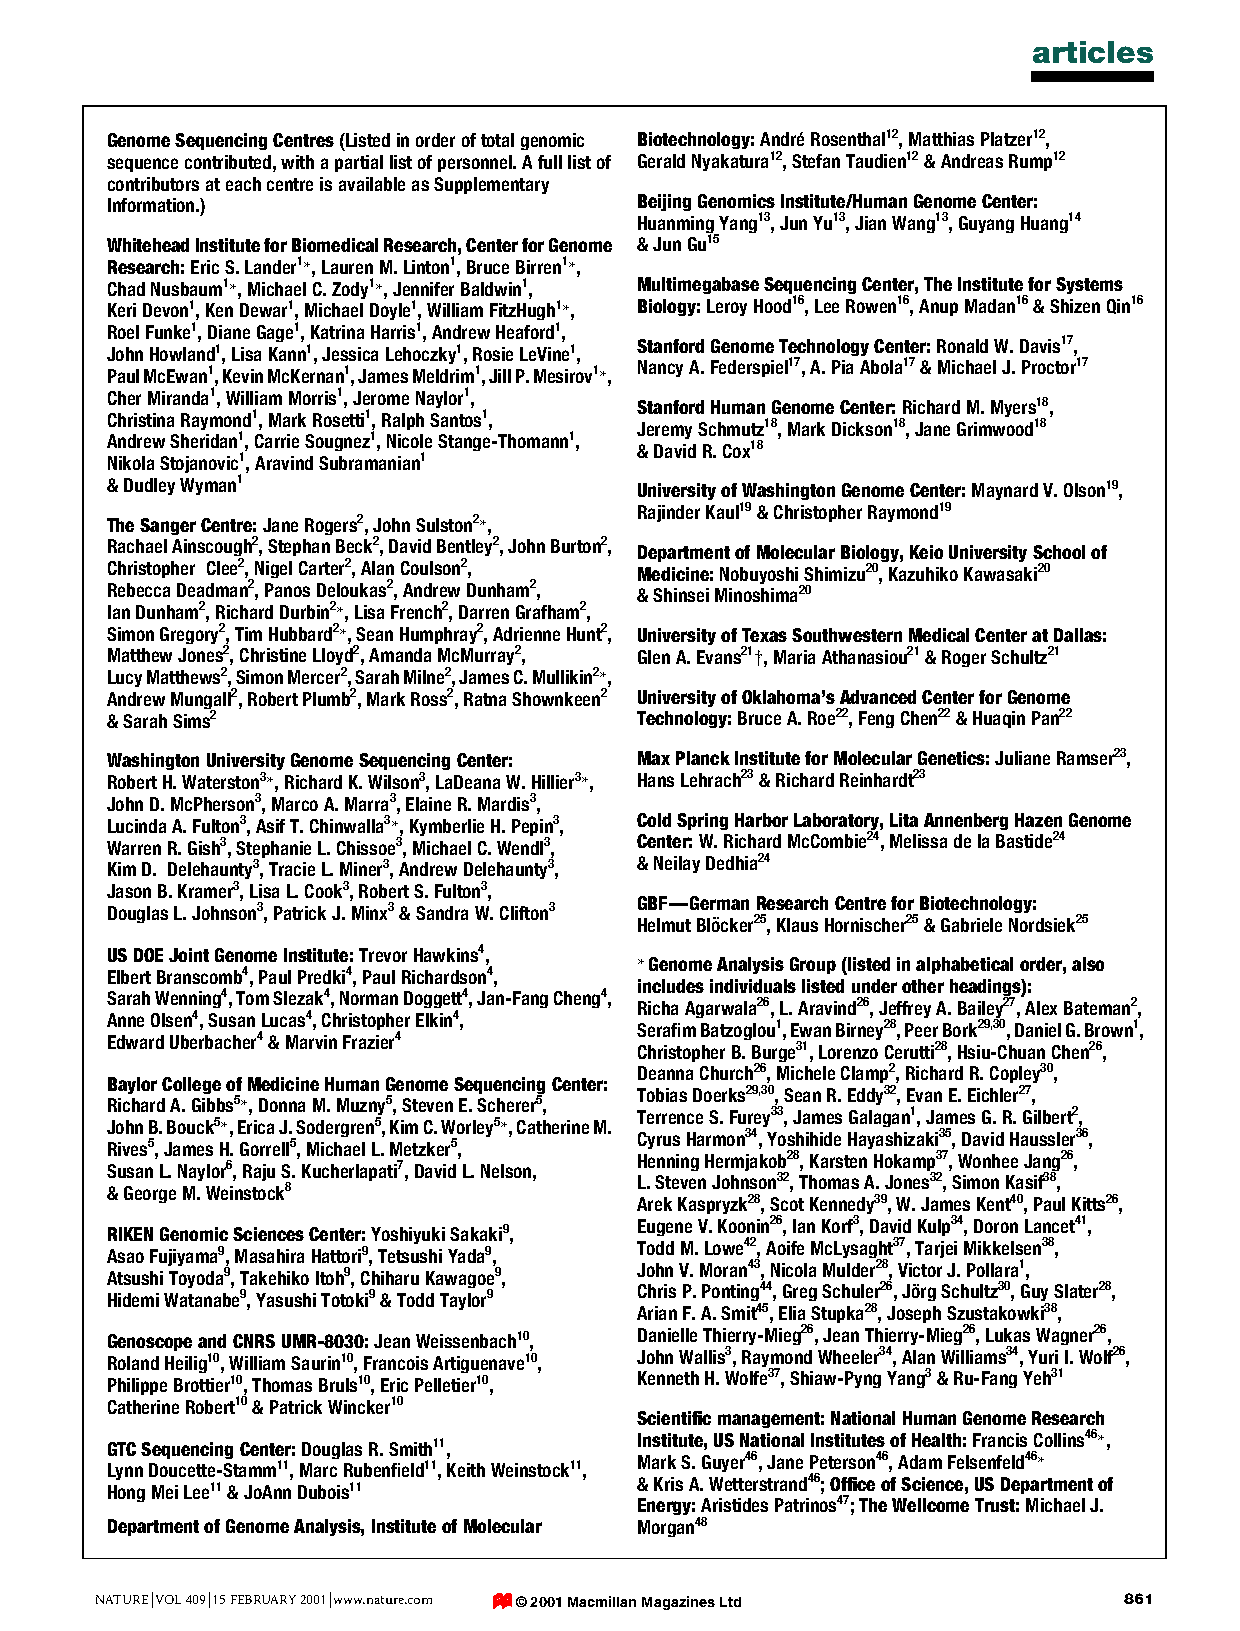
\includegraphics[height=\textheight]{figures/lander_initial_2001_authors}
\end{center}

\end{frame}
%%%%%%%%%%%%%%%%%%%%%%%%%%
\begin{frame}

\begin{center}
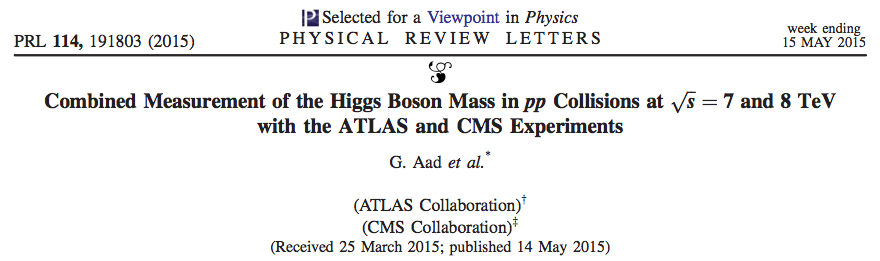
\includegraphics[width=\textwidth]{figures/aad_combined_2015_title}
\end{center}

\vfill
{\tiny \url{https://doi.org/10.1103/PhysRevLett.114.191803}}

\end{frame}
%%%%%%%%%%%%%%%%%%%%%%%%%%
\begin{frame}

\begin{center}
\includegraphics[height=\textheight]<1>{figures/aad_combined_2015_authors_01}
\includegraphics[height=\textheight]<2>{figures/aad_combined_2015_authors_02}
\includegraphics[height=\textheight]<3>{figures/aad_combined_2015_authors_03}
\includegraphics[height=\textheight]<4>{figures/aad_combined_2015_authors_04}
\includegraphics[height=\textheight]<5>{figures/aad_combined_2015_authors_05}
\includegraphics[height=\textheight]<6>{figures/aad_combined_2015_authors_06}
\includegraphics[height=\textheight]<7>{figures/aad_combined_2015_authors_07}
\includegraphics[height=\textheight]<8>{figures/aad_combined_2015_authors_08}
\includegraphics[height=\textheight]<9>{figures/aad_combined_2015_authors_09}
\includegraphics[height=\textheight]<10>{figures/aad_combined_2015_authors_10}
\includegraphics[height=\textheight]<11>{figures/aad_combined_2015_authors_11}
\includegraphics[height=\textheight]<12>{figures/aad_combined_2015_authors_12}
\includegraphics[height=\textheight]<13>{figures/aad_combined_2015_authors_13}
\includegraphics[height=\textheight]<14>{figures/aad_combined_2015_authors_14}
\includegraphics[height=\textheight]<15>{figures/aad_combined_2015_authors_15}
\includegraphics[height=\textheight]<16>{figures/aad_combined_2015_authors_16}
\includegraphics[height=\textheight]<17>{figures/aad_combined_2015_authors_17}
\includegraphics[height=\textheight]<18>{figures/aad_combined_2015_authors_18}
\includegraphics[height=\textheight]<19>{figures/aad_combined_2015_authors_19}
\includegraphics[height=\textheight]<20>{figures/aad_combined_2015_authors_20}
\includegraphics[height=\textheight]<21>{figures/aad_combined_2015_authors_21}
\includegraphics[height=\textheight]<22>{figures/aad_combined_2015_authors_22}
\includegraphics[height=\textheight]<23>{figures/aad_combined_2015_authors_23}
\includegraphics[height=\textheight]<24>{figures/aad_combined_2015_authors_24}
\includegraphics[height=\textheight]<25>{figures/aad_combined_2015_authors_25}
\end{center}

\end{frame}
%%%%%%%%%%%%%%%%%%%%%%%%%
\begin{frame}

\begin{center}
\Large{Fragile Families Challenge} \pause
\end{center}
A scientific mass collaboration combining \pause
\begin{itemize}
\item predictive modeling,\pause 
\item causal inference, \pause 
\item and qualitative interviews 
\end{itemize}
\pause to improve the lives of disadvantaged children in the US.  

\end{frame}
%%%%%%%%%%%%%%%%%%%%%%%%%%%
\begin{frame}

\begin{center}

\includegraphics[width=\textwidth]{figures/ff_logo}
\end{center}

\begin{itemize}
\item Birth cohort panel study
\item $\approx$ 5,000 children born in 20 U.S. cities
\item Oversample of non-marital births 
\item Followed from birth through age 15
\end{itemize}

\textcolor{blue}{Key research question}: What can be done to improve the life chances of disadvantaged children?

\end{frame}
%%%%%%%%%%%%%%%%%%%%%%%%%%%
\begin{frame}

Hundreds of papers and dozens of dissertations \vskip 1cm
\scriptsize \url{http://crcw.princeton.edu/publications/publications.asp}

\end{frame}
%%%%%%%%%%%%%%%%%%%%%%%%%%
\begin{frame}

\begin{center}
\includegraphics[width=\textwidth]<1>{figures/ffPub1}
\includegraphics[width=\textwidth]<2>{figures/ffPub2}
\includegraphics[width=\textwidth]<3>{figures/ffPub3}
\includegraphics[width=\textwidth]<4>{figures/ffPub4}
\includegraphics[width=\textwidth]<5>{figures/ffPub5}
\end{center}

\end{frame}
%%%%%%%%%%%%%%%%%%%%%%%%%
\begin{frame}

\begin{center}
\large{Social Scientists $\longleftrightarrow$ Data Scientists}
\end{center}
\pause
\begin{center}
\LARGE{
$\hat{\beta} \quad \& \quad \hat{y}$
}
\end{center}

\end{frame}
%%%%%%%%%%%%%%%%%%%%%%%%%
\begin{frame}

\begin{center}
\only<1>{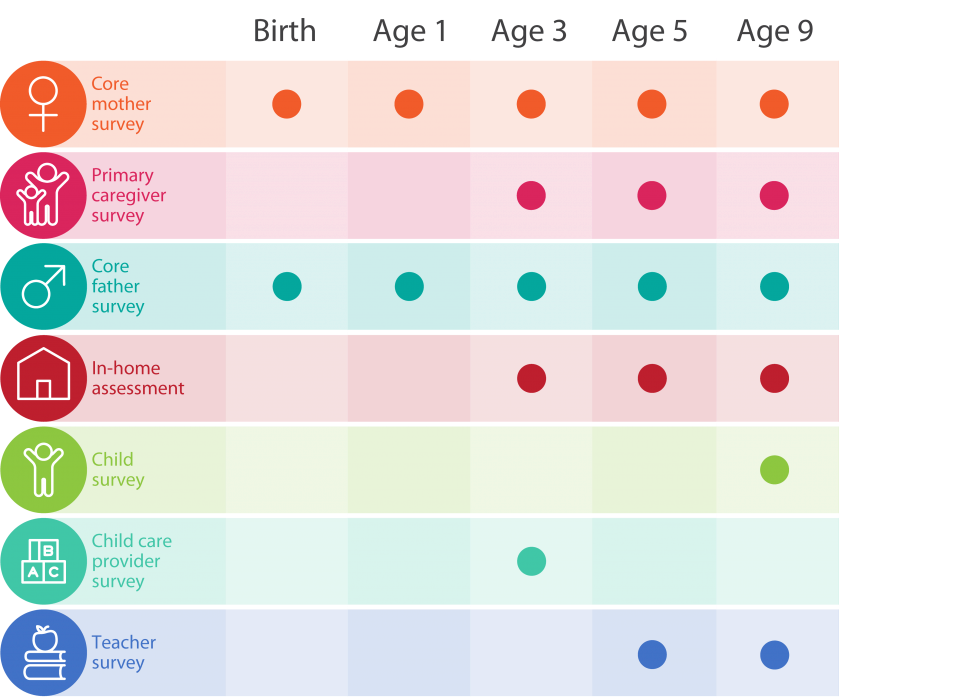
\includegraphics[width=\textwidth]{figures/ff_design_public_b9}}
\only<2>{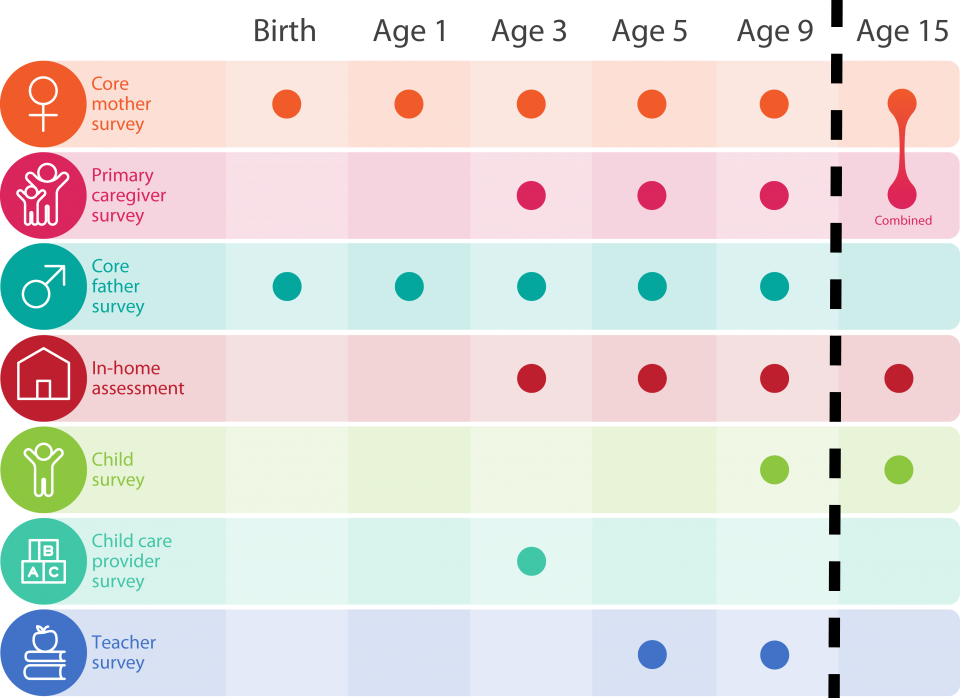
\includegraphics[width=\textwidth]{figures/ff_design_public2}}
\end{center}

\end{frame}
%%%%%%%%%%%%%%%%%%%%%%%%%
\begin{frame}

\begin{center}
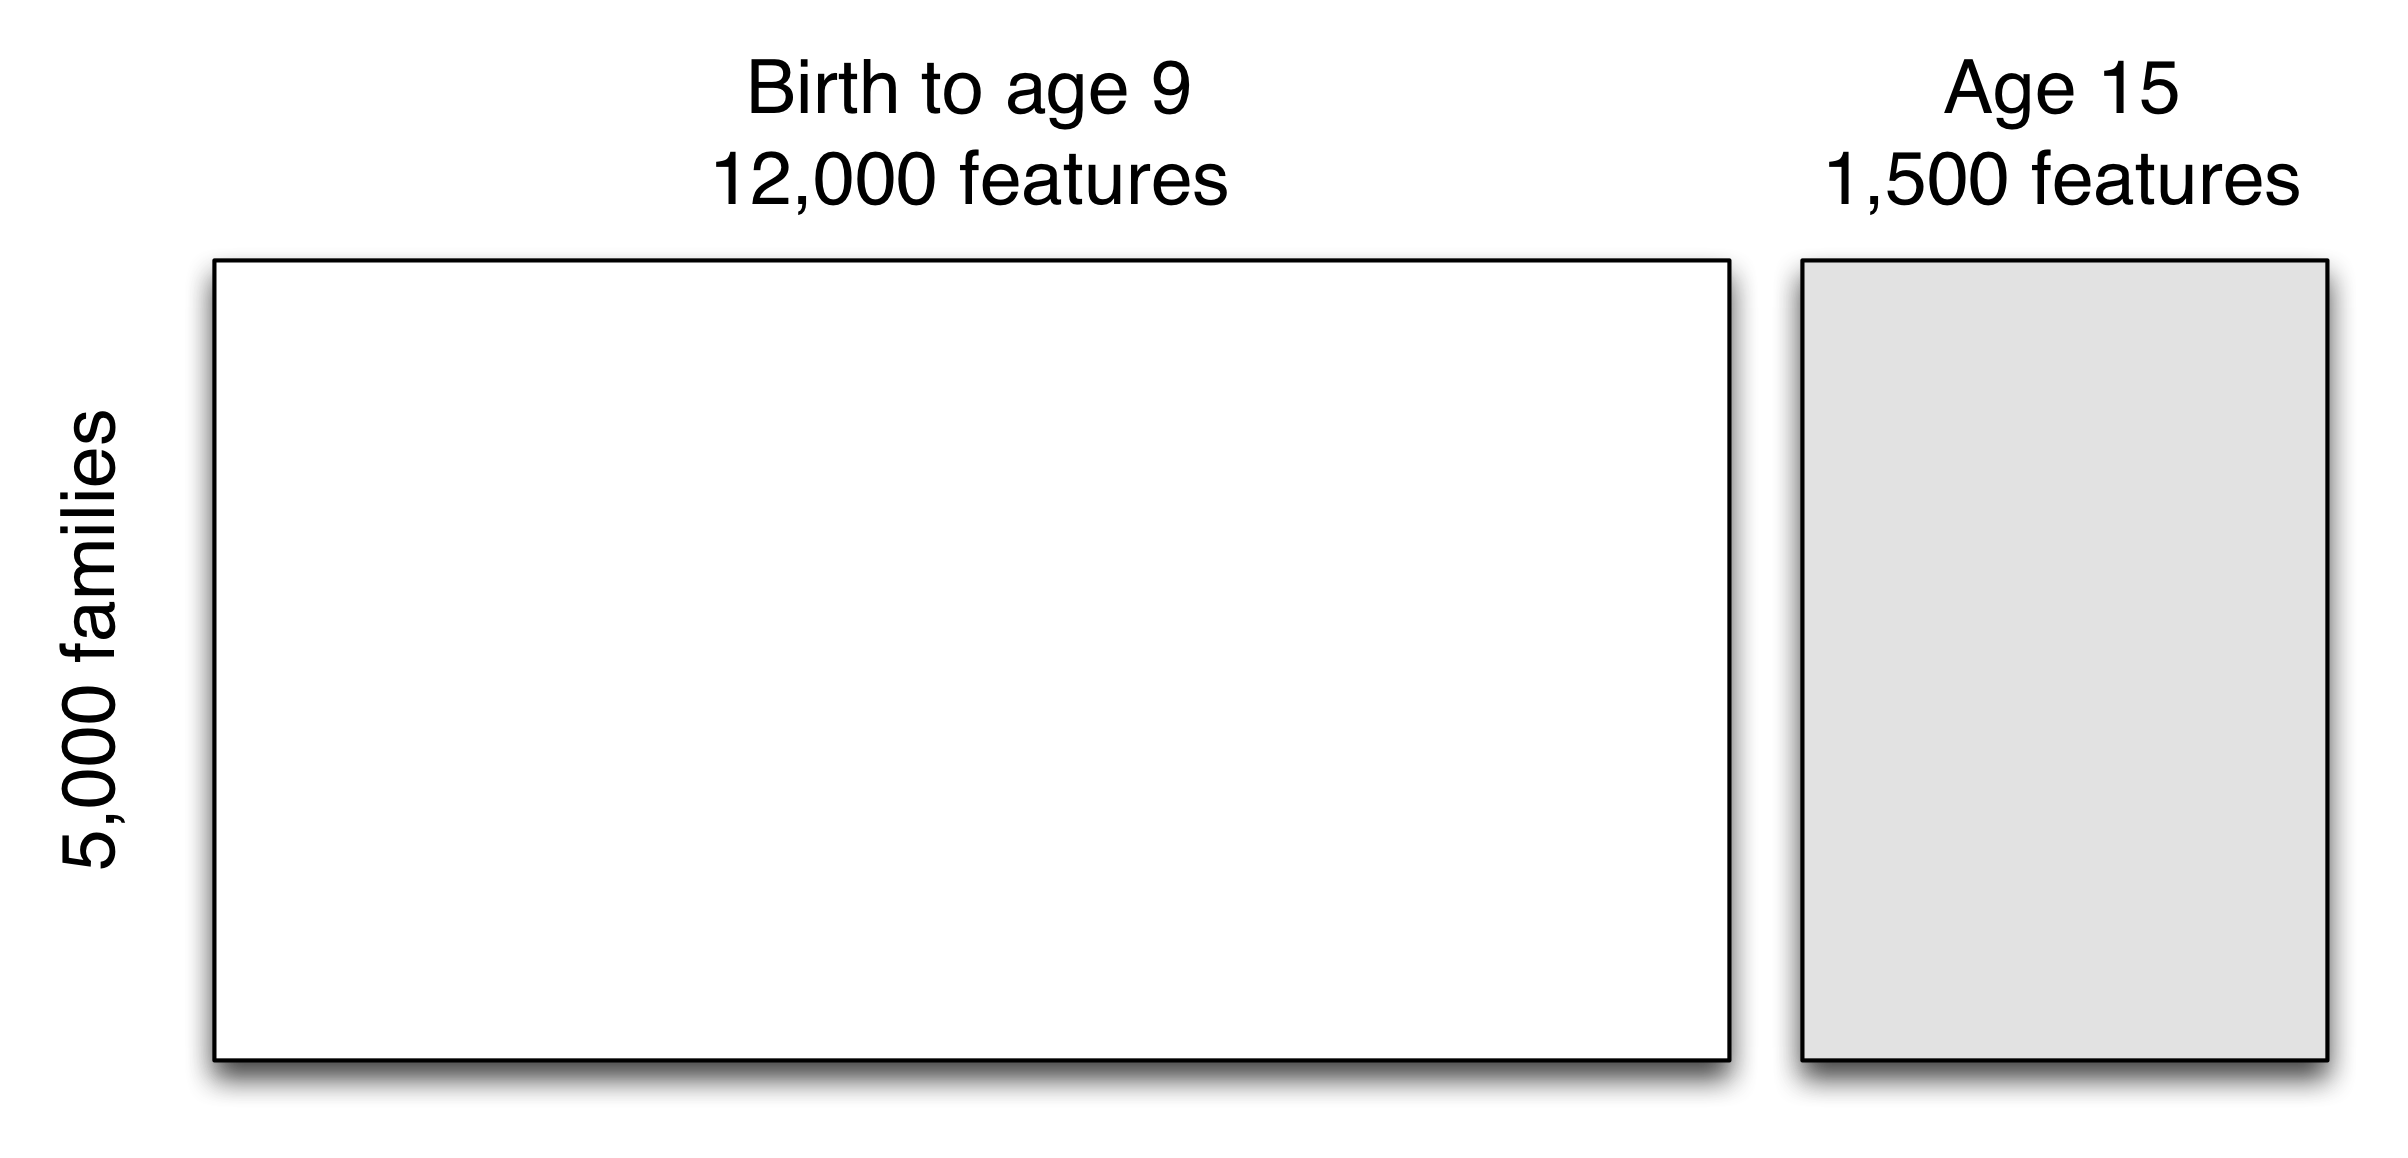
\includegraphics[width=\textwidth]{figures/ff_design_matrix_ml}
\end{center}

\end{frame}
%%%%%%%%%%%%%%%%%%%%%%%%%
\begin{frame}

\begin{center}
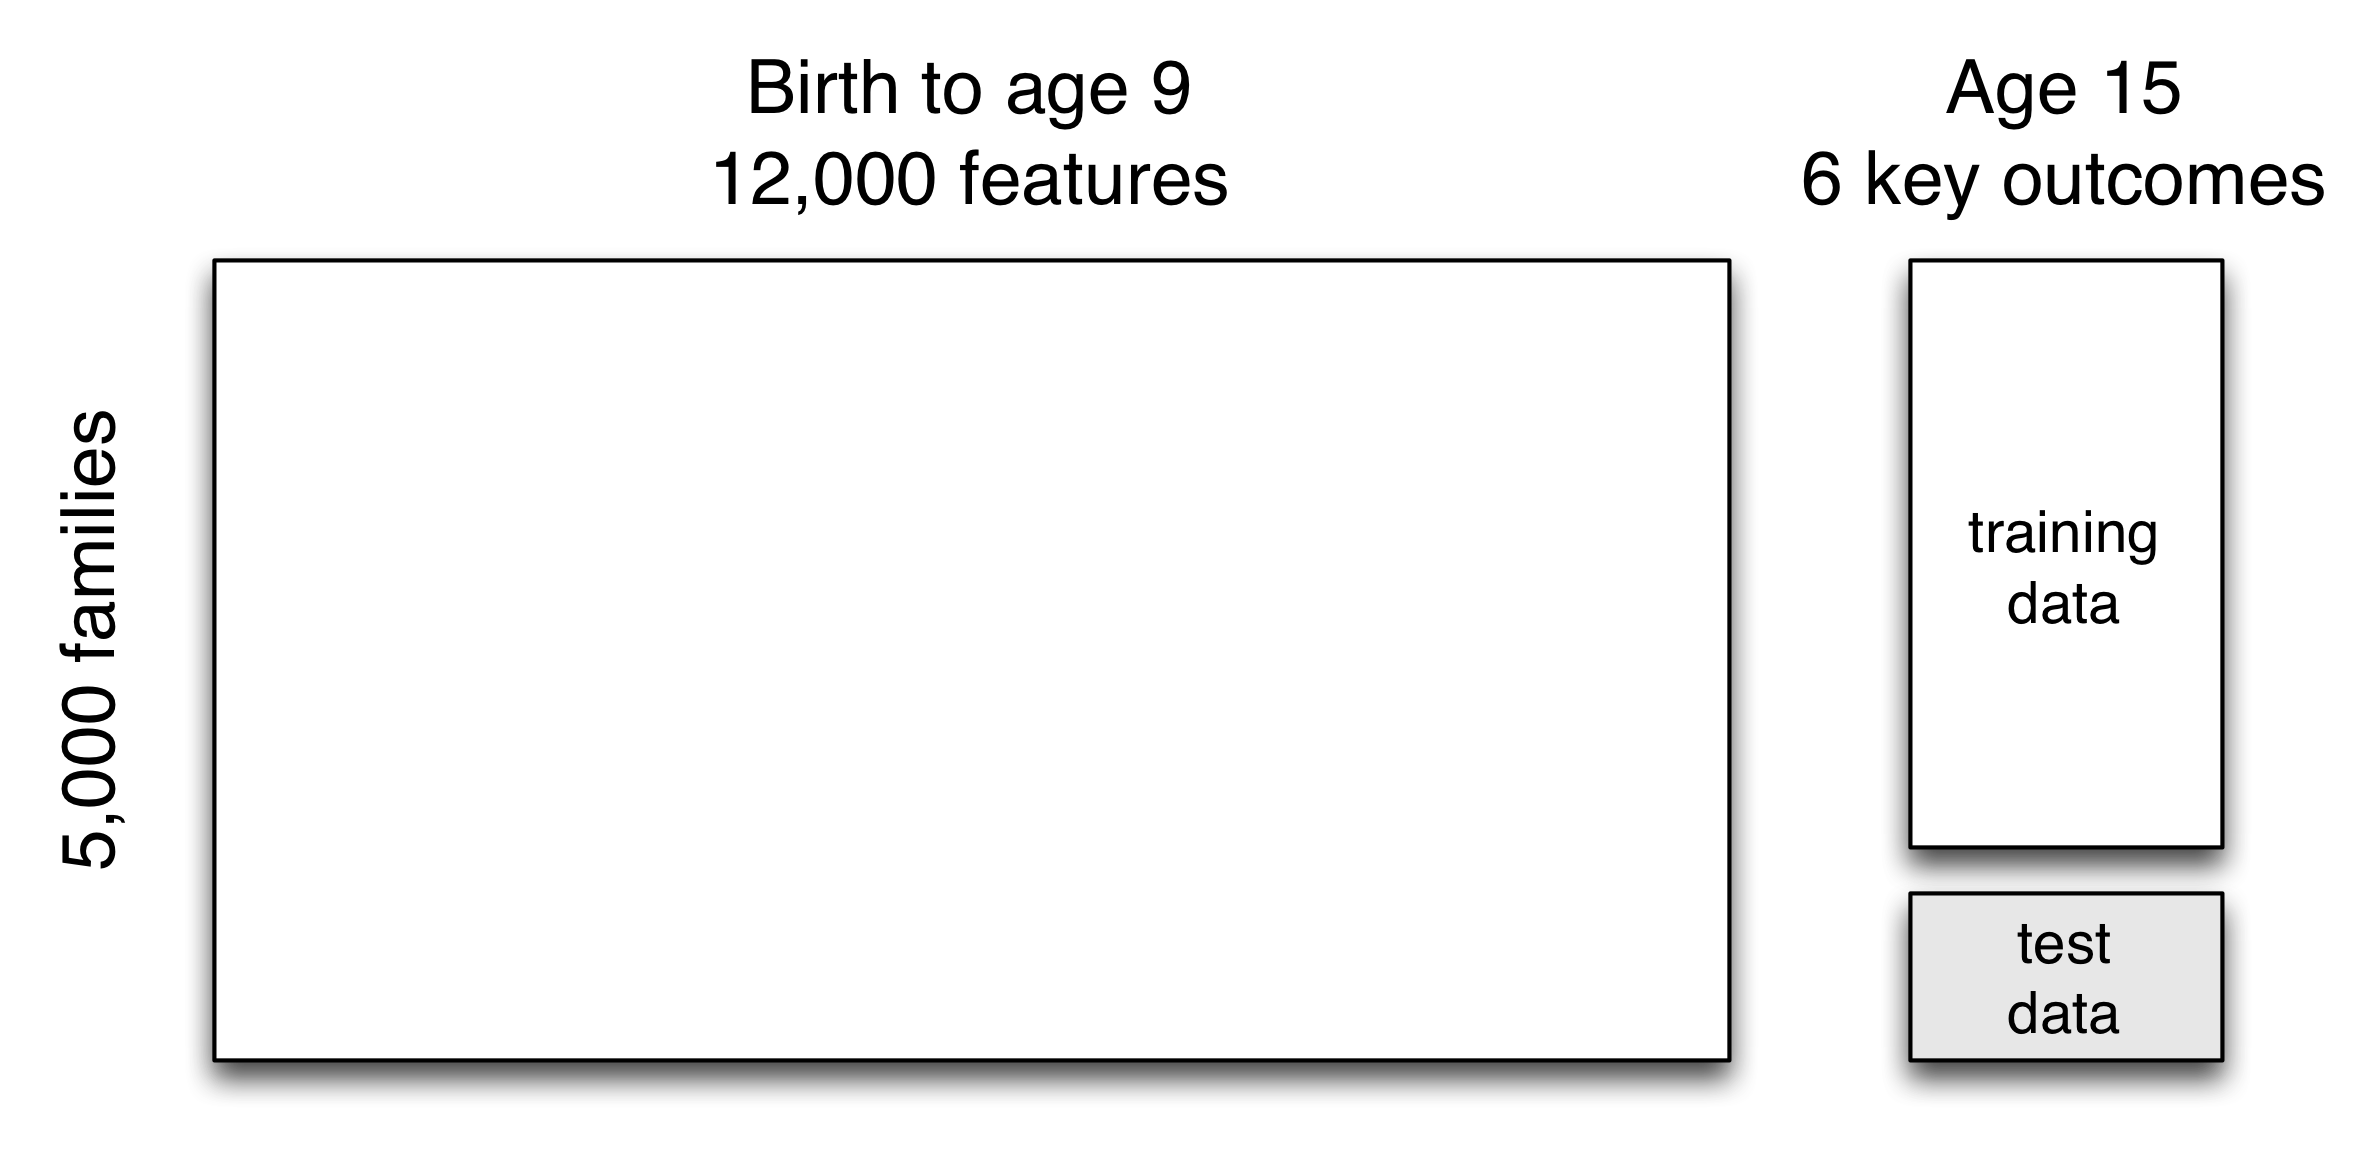
\includegraphics[width=\textwidth]{figures/challenge_design_matrix}
\end{center}

\end{frame}
%%%%%%%%%%%%%%%%%%%%%%%%%
\begin{frame}

\begin{tabular}{p{.4\textwidth}p{.4\textwidth}}
Continuous outcomes:
\begin{itemize}
\item GPA
\item Grit
\item Material hardship
\end{itemize}
&
Binary outcomes:
\begin{itemize}
\item Housing eviction
\item Layoff of a caregiver
\item Job training for a caregiver
\end{itemize}
\end{tabular}

\end{frame}
%%%%%%%%%%%%%%%%%%%%%%%%%
\begin{frame}

Fragile Families Challenge:
\begin{enumerate}
\item common task method
\pause
\item use submissions to do cool stuff
\end{enumerate}

\end{frame}
%%%%%%%%%%%%%%%%%%%%%%%%%
\begin{frame}

Common task method
\begin{itemize}
\item common data
\item common metric
\item evaluation on held-out test data
\end{itemize}

``secret sauce'' of machine learning (Donoho 2015)

\end{frame}
%%%%%%%%%%%%%%%%%%%%%%%%%
\begin{frame}

\begin{center}
\only<1>{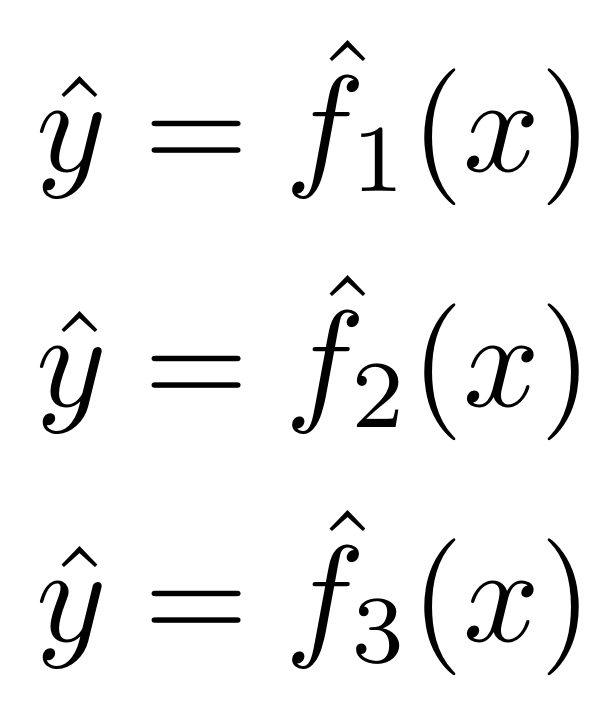
\includegraphics[width=0.3\textwidth]{figures/ff_ensemble_1}}
\only<2>{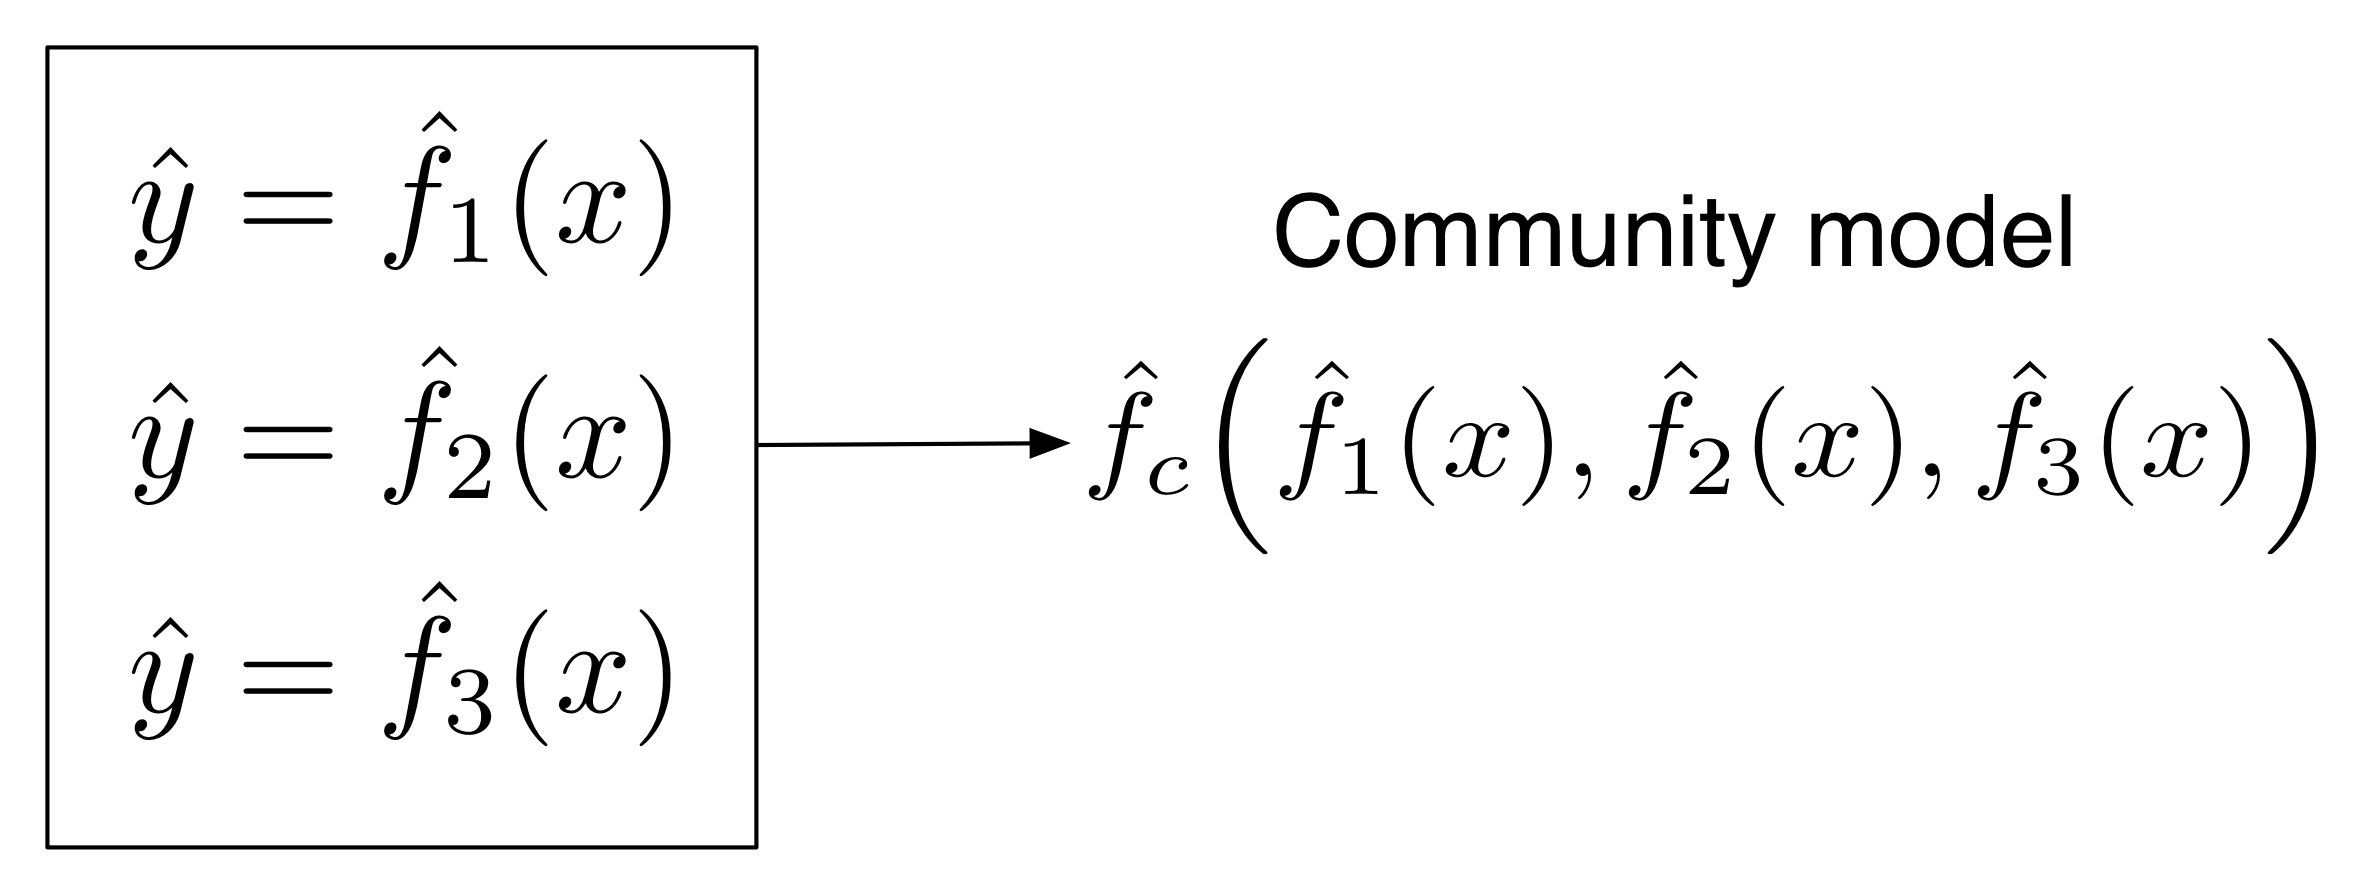
\includegraphics[width=0.8\textwidth]{figures/ff_ensemble_2}}
\only<3>{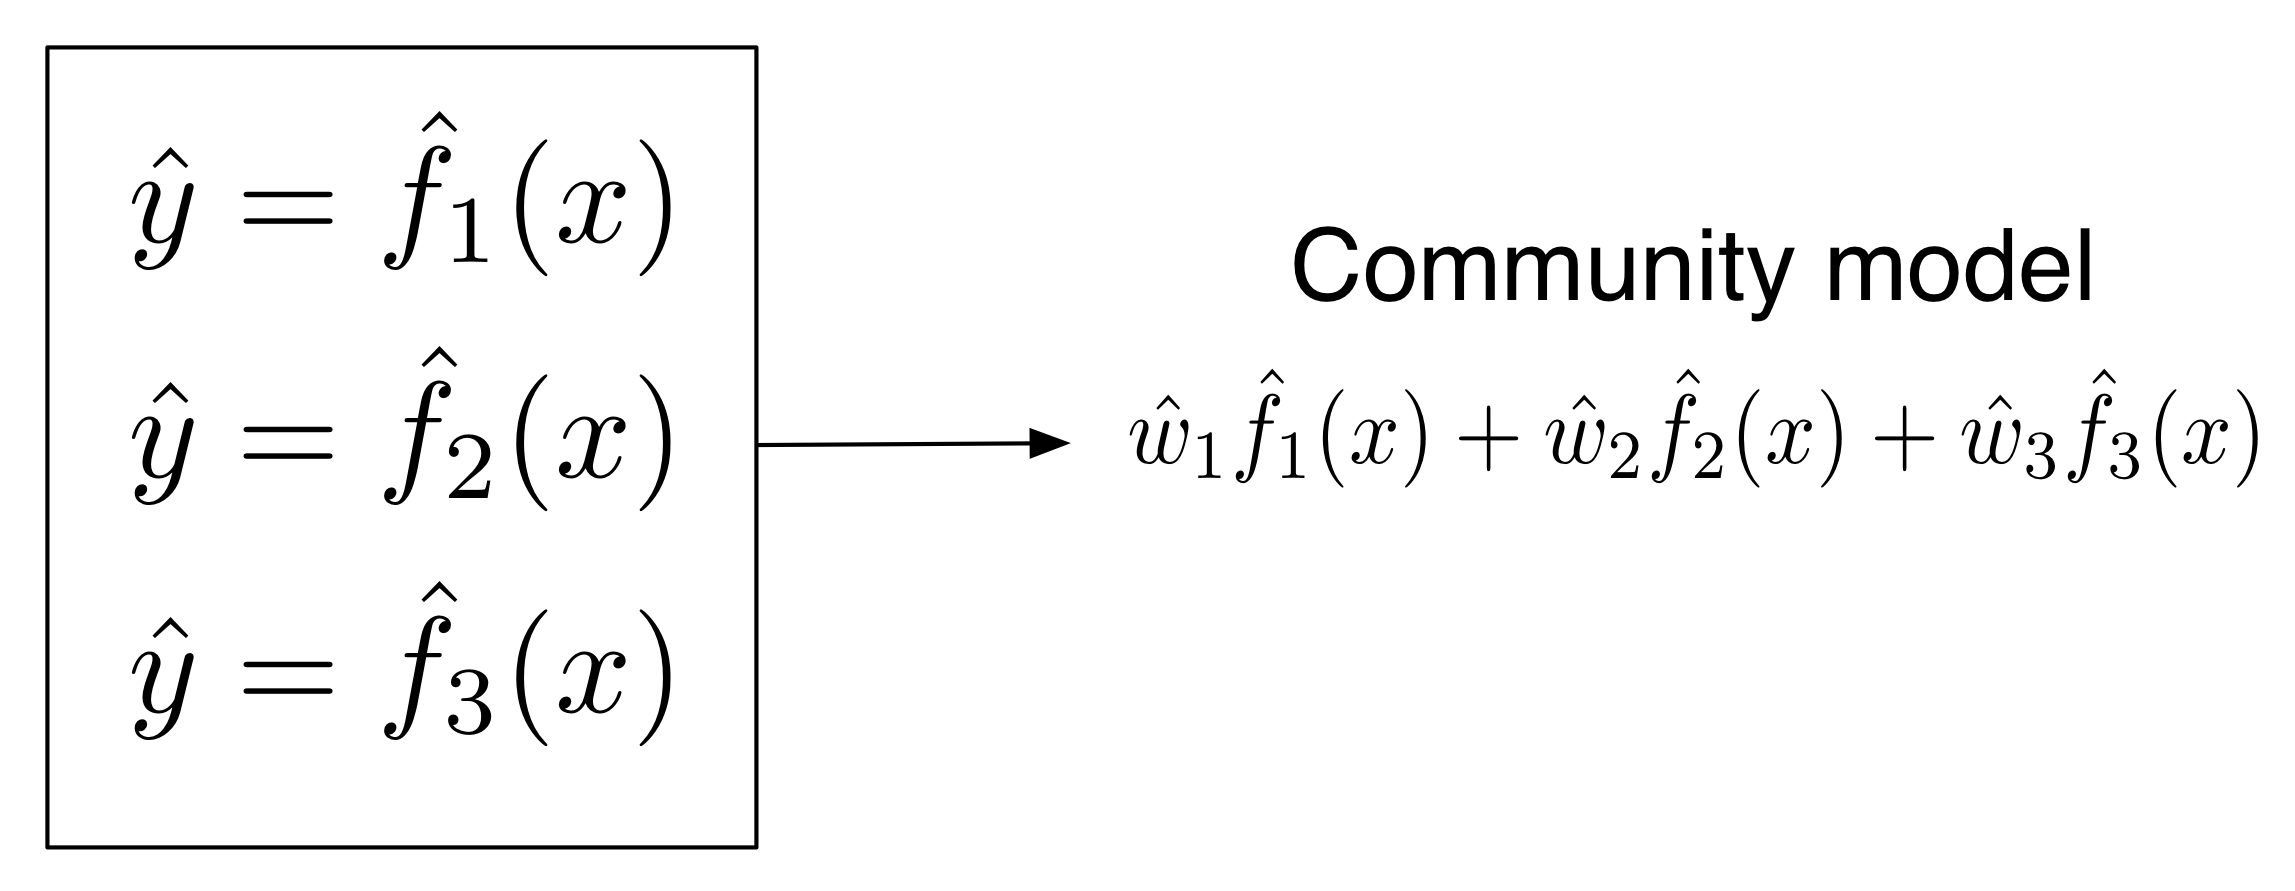
\includegraphics[width=0.8\textwidth]{figures/ff_ensemble_3}}
\end{center}

\end{frame}
%%%%%%%%%%%%%%%%%%%%%%%%%
\begin{frame}

\begin{center}
\Large{
What's so special about this community model?
}
\end{center}

\end{frame}
%%%%%%%%%%%%%%%%%%%%%%%%%
\begin{frame}

Use community model to
\begin{itemize}
\item look for ``dark matter''
\item estimate causal effects
\end{itemize}

\end{frame}
%%%%%%%%%%%%%%%%%%%%%%%%%
\begin{frame}

Use community model to
\begin{itemize}
\item \textcolor{blue}{look for ``dark matter''}\footnote{Learn more at \url{http://www.fragilefamilieschallenge.org/unmeasured-factors/}\vskip .2cm}
\item estimate causal effects
\end{itemize}

\end{frame}
%%%%%%%%%%%%%%%%%%%%%%%%%
\begin{frame}

Most social science models have poor predictive performance.  Why?

\pause
\begin{itemize}
\item poor measurement
\pause
\item wrong functional form
\pause
\item ``dark matter''
\end{itemize}

\end{frame}
%%%%%%%%%%%%%%%%%%%%%%%%%
\begin{frame}

Look for dark matter:
\begin{itemize}
\item Interview kids and families that are beating the odds (and not)
\pause
\item Three continuous outcomes: GPA, Material Hardship, Grit
\pause
\item Machine learning in the service of in-depth interviews
\end{itemize}

\end{frame}
%%%%%%%%%%%%%%%%%%%%%%%%%
\begin{frame}

Use community model to
\begin{itemize}
\item \textcolor{blue}{look for ``dark matter''}
\item estimate causal effects
\end{itemize}

\end{frame}
%%%%%%%%%%%%%%%%%%%%%%%%%
\begin{frame}

Use community model to
\begin{itemize}
\item look for ``dark matter''
\item \textcolor{blue}{estimate causal effects}\footnote{Learn more at \url{http://www.fragilefamilieschallenge.org/causal-inference/}\vskip .2cm}
\end{itemize}

\end{frame}
%%%%%%%%%%%%%%%%%%%%%%%%%
\begin{frame}

\begin{center}
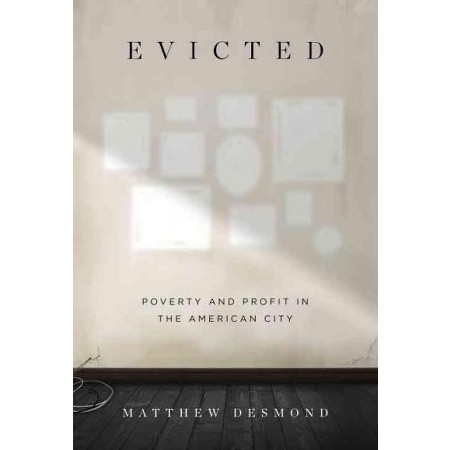
\includegraphics[height = .9\textheight]{figures/desmond_evicted_2016_cover}
\end{center}

\end{frame}
%%%%%%%%%%%%%%%%%%%%%%%%%
\begin{frame}

Does eviction \textcolor{blue}{cause} children's outcomes to be worse? \vskip .5cm \pause
Or is eviction just \textcolor{blue}{associated with} worse outcomes because those who are evicted are already disadvantaged in other ways?

\end{frame}
%%%%%%%%%%%%%%%%%%%%%%%%%
\begin{frame}

\begin{center}
\begin{tikzpicture}
  \node (T) at (0,0) {$T$ = Eviction};
  \node (Y) at (4, 0) {$Y$ = Child outcomes};
  \node (Ut) at (0, 2) {$U_T$};
  \node (X) at (-4, 0) {$X$};
  \draw[->, >=stealth, thick] (T) -- (Y);
  \draw[->, >=stealth, thick] (X) -- (T);
  \draw[->, >=stealth, thick] (X) to[bend right]  (Y);
  \draw[->, >=stealth, thick] (Ut) --  (T);
  %\draw[->, >=stealth, thick, dashed] (Ut) --  (Y);
\end{tikzpicture}
\end{center}

\end{frame}
%%%%%%%%%%%%%%%%%%%%%%%%%
\begin{frame}

\begin{center}
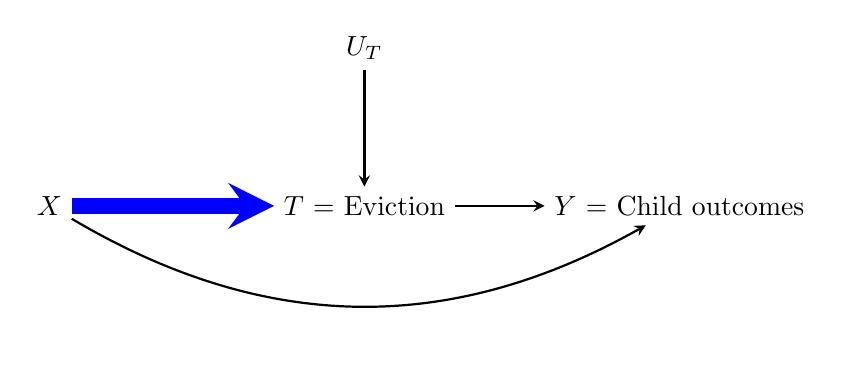
\begin{tikzpicture}
  \node (T) at (0,0) {$T$ = Eviction};
  \node (Y) at (4, 0) {$Y$ = Child outcomes};
  \node (Ut) at (0, 2) {$U_T$};
  \node (X) at (-4, 0) {$X$};
  \draw[->, >=stealth, thick] (T) -- (Y);
  \draw[->, >=stealth, line width = 6pt, blue] (X) -- (T);
  \draw[->, >=stealth, thick] (X) to[bend right]  (Y);
  \draw[->, >=stealth, thick] (Ut) --  (T);
  %\draw[->, >=stealth, thick, dashed] (Ut) --  (Y);
\end{tikzpicture}
\end{center}

\end{frame}
%%%%%%%%%%%%%%%%%%%%%%%%%
\begin{frame}

\begin{center}
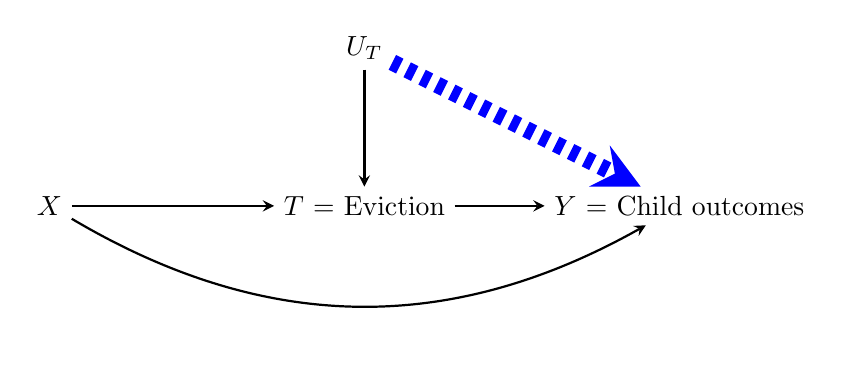
\begin{tikzpicture}
  \node (T) at (0,0) {$T$ = Eviction};
  \node (Y) at (4, 0) {$Y$ = Child outcomes};
  \node (Ut) at (0, 2) {$U_T$};
  \node (X) at (-4, 0) {$X$};
  \draw[->, >=stealth, thick] (T) -- (Y);
  \draw[->, >=stealth, thick] (X) -- (T);
  \draw[->, >=stealth, thick] (X) to[bend right]  (Y);
  \draw[->, >=stealth, thick] (Ut) --  (T);
  \draw[->, >=stealth, blue, line width = 6pt, dashed] (Ut) --  (Y);
\end{tikzpicture}
\end{center}

\end{frame}
%%%%%%%%%%%%%%%%%%%%%%%%%
\begin{frame}

Causal inference from observational data is hard but important
\pause
\begin{itemize}
\item Community model produces propensity scores used for matching
\pause
\item Sensitivity analysis
\pause
\item In-depth interviews to check assumption of selection on observables
\end{itemize}

\end{frame}
%%%%%%%%%%%%%%%%%%%%%%%%%
\begin{frame}

Use community model to
\begin{itemize}
\item look for ``dark matter''
\item estimate causal effects
\end{itemize}

\end{frame}
%%%%%%%%%%%%%%%%%%%%%%%%%
\begin{frame}

\begin{center}
To enable future research,\\at the end of the Challenge,\\we will \textcolor{blue}{open-source} all submitted\\predictions, code, and narrative explanations.
\vskip .5cm \pause
Some participants have \textcolor{blue}{already} provided \\ open source examples submissions! \\ \vskip .2cm
\begin{large}\textcolor{blue}{\url{http://github.com/fragilefamilieschallenge/open-source-submissions}}\end{large}
\end{center}

\end{frame}
%%%%%%%%%%%%%%%%%%%%%%%%%%%
\section{How to participate}
%%%%%%%%%%%%%%%%%%%%%%%%%
\begin{frame}

\large{
\begin{center}
How to participate \vskip .5cm
\textcolor{blue}{\href{http://www.fragilefamilieschallenge.org}{www.fragilefamilieschallenge.org}}
\end{center}
}

\end{frame}
%%%%%%%%%%%%%%%%%%%%%%%%%
\begin{frame}

\Large{
\begin{center}
Introducing the outcome variables
\end{center}
}

\end{frame}
%%%%%%%%%%%%%%%%%%%%%%%%%
\begin{frame}

\Large{
\begin{center}
GPA\footnote{Learn more at \url{http://www.fragilefamilieschallenge.org/gpa/} \vskip .2cm}
\pause \vskip .5cm
How do kids beat the odds academically?
\end{center}
}

\end{frame}
%%%%%%%%%%%%%%%%%%%%%%%%%
\begin{frame}{GPA\footnote{This variable is reverse-coded in the data file so that higher values represent higher GPAs.}}

\centering
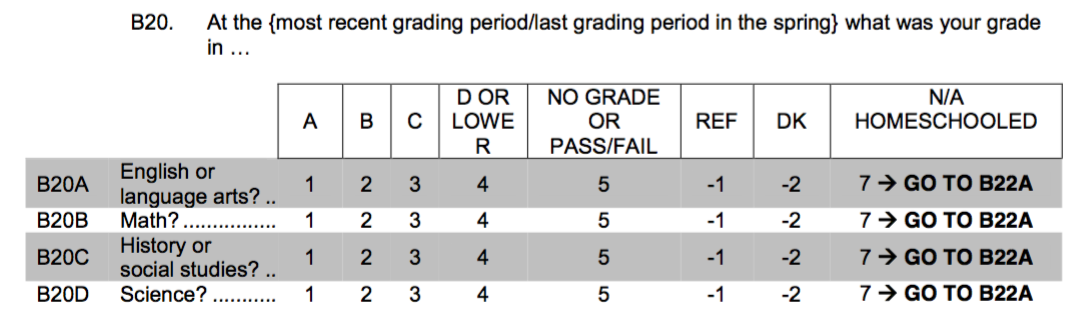
\includegraphics[width = .9\textwidth]{figures/GPA_questionnaire}

\end{frame}
%%%%%%%%%%%%%%%%%%%%%%%%%
\begin{frame}

\centering
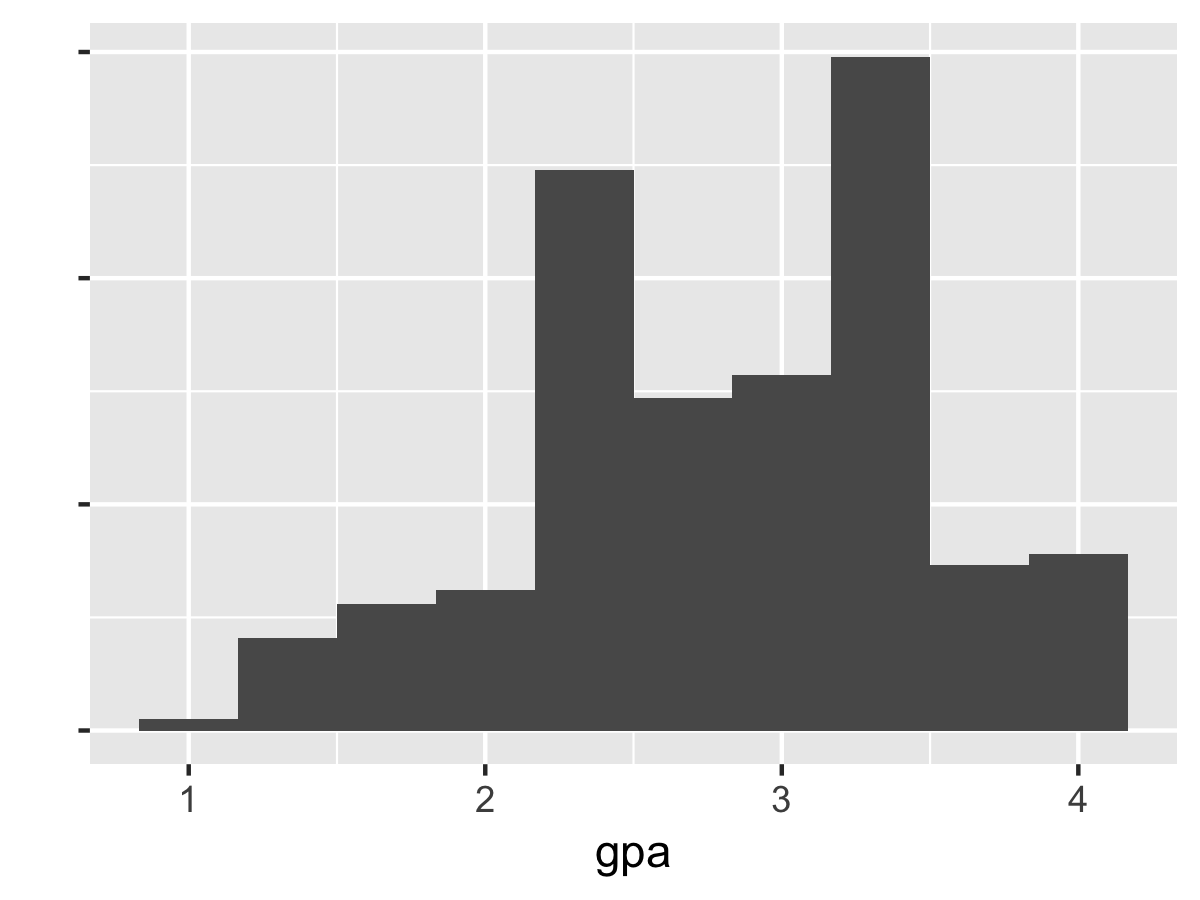
\includegraphics[width = .9\textwidth]{figures/gpaDist}

\end{frame}
%%%%%%%%%%%%%%%%%%%%%%%%%
\begin{frame}
\begin{center}
\Large{
``Grit'' predicts success, possibly more than IQ.\footnote{Learn more at \url{http://www.fragilefamilieschallenge.org/grit/}\vskip .2cm} \vskip .3cm

\includegraphics[width = .3\textwidth]{figures/duckworth_grit_2016_cover} \vskip .3cm \pause
What makes some kids gritty?
} 
\end{center}
\end{frame}
%%%%%%%%%%%%%%%%%%%%%%%%%%%
\begin{frame}{Grit\footnote{This variable is reverse-coded in the data file so that higher values represent more grit.}}

\centering
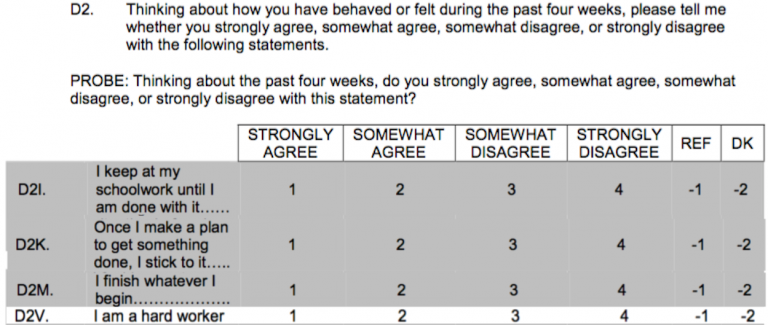
\includegraphics[width = .9\textwidth]{figures/grit_questionnaire2}

\end{frame}
%%%%%%%%%%%%%%%%%%%%%%%%%
\begin{frame}

\centering
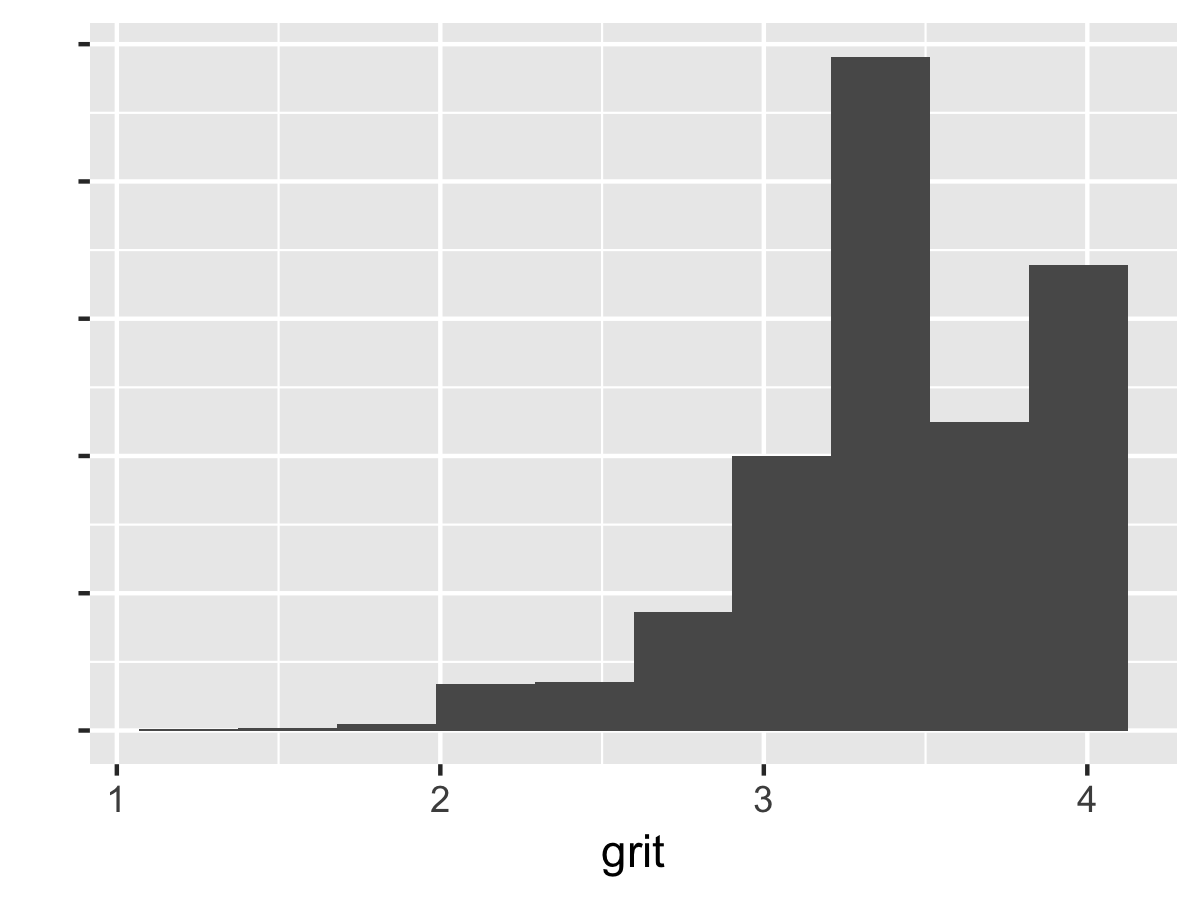
\includegraphics[width = .9\textwidth]{figures/gritDist}

\end{frame}
%%%%%%%%%%%%%%%%%%%%%%%%%
\begin{frame}

\Large{
\begin{center}
Material hardship\footnote{Learn more at \url{http://www.fragilefamilieschallenge.org/material-hardship/}\vskip .2cm} \pause \vskip .3cm 
What unmeasured predictors are associated with families unexpectedly escaping severe deprivation? 
\pause \vskip .3cm What sends families unexpectedly into deep poverty?
\end{center}
}

\end{frame}
%%%%%%%%%%%%%%%%%%%%%%%%%%%
\begin{frame}{Material hardship}

\centering
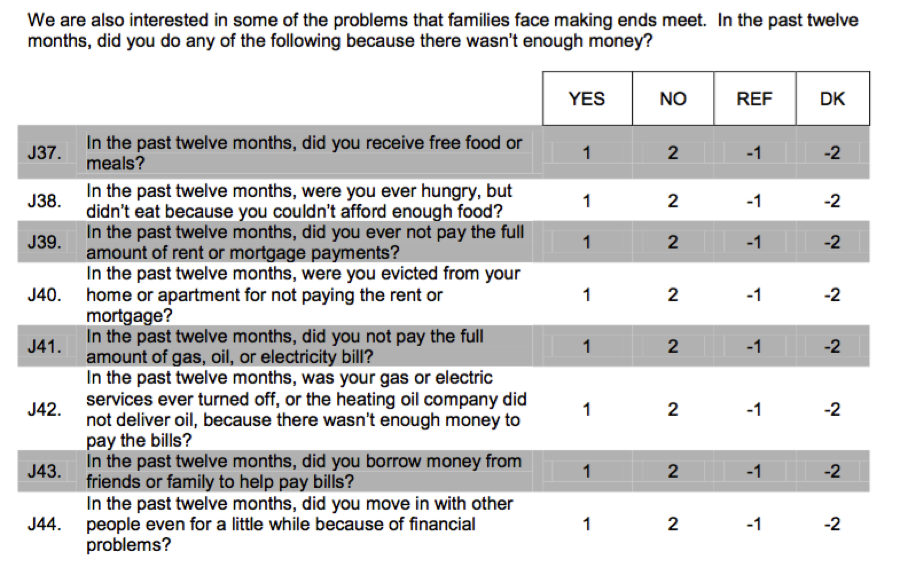
\includegraphics[width = .9\textwidth]{figures/materialHardship_questionnaireA}

\end{frame}
%%%%%%%%%%%%%%%%%%%%%%%%%%%
\begin{frame}{Material hardship}

\centering
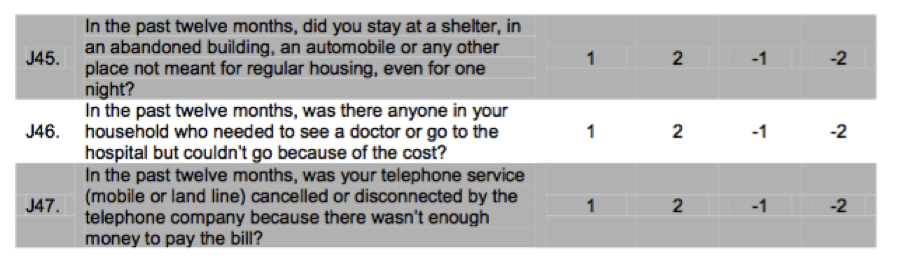
\includegraphics[width = .9\textwidth]{figures/materialHardship_questionnaireB}

\end{frame}
%%%%%%%%%%%%%%%%%%%%%%%%%
\begin{frame}

\centering
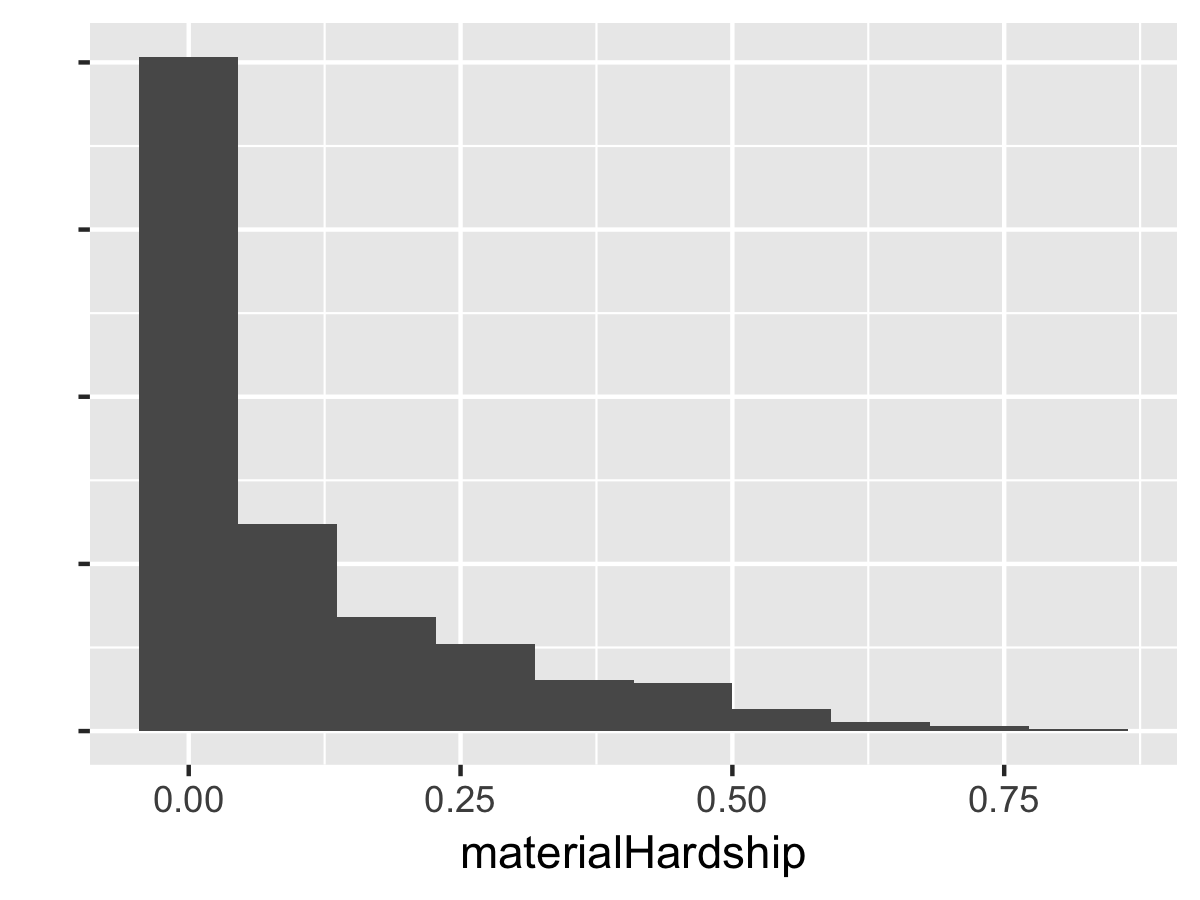
\includegraphics[width = .9\textwidth]{figures/materialHardshipDist}

\end{frame}
%%%%%%%%%%%%%%%%%%%%%%%%%
\begin{frame}

\Large{
\begin{center}
Eviction\footnote{Learn more at \url{http://www.fragilefamilieschallenge.org/eviction/}\vskip .2cm}
\pause \vskip .5cm
Does housing eviction \textbf{cause} worse outcomes as kids transition to adulthood?\footnote{Note: You will just create propensity scores for eviction given background variables; causal inference comes in the second stage of the Challenge when outcomes are measured several years from now.}
\end{center}
}

\end{frame}
%%%%%%%%%%%%%%%%%%%%%%%%%%%
\begin{frame}{Eviction}

\centering
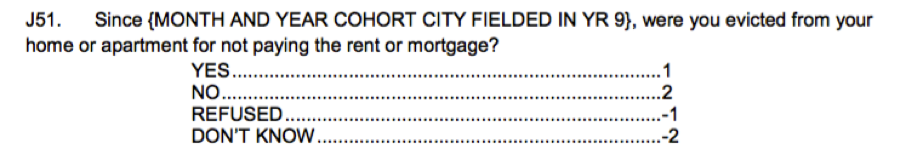
\includegraphics[width = .9\textwidth]{figures/eviction_questionnaire}

\end{frame}
%%%%%%%%%%%%%%%%%%%%%%%%%
\begin{frame}

\centering
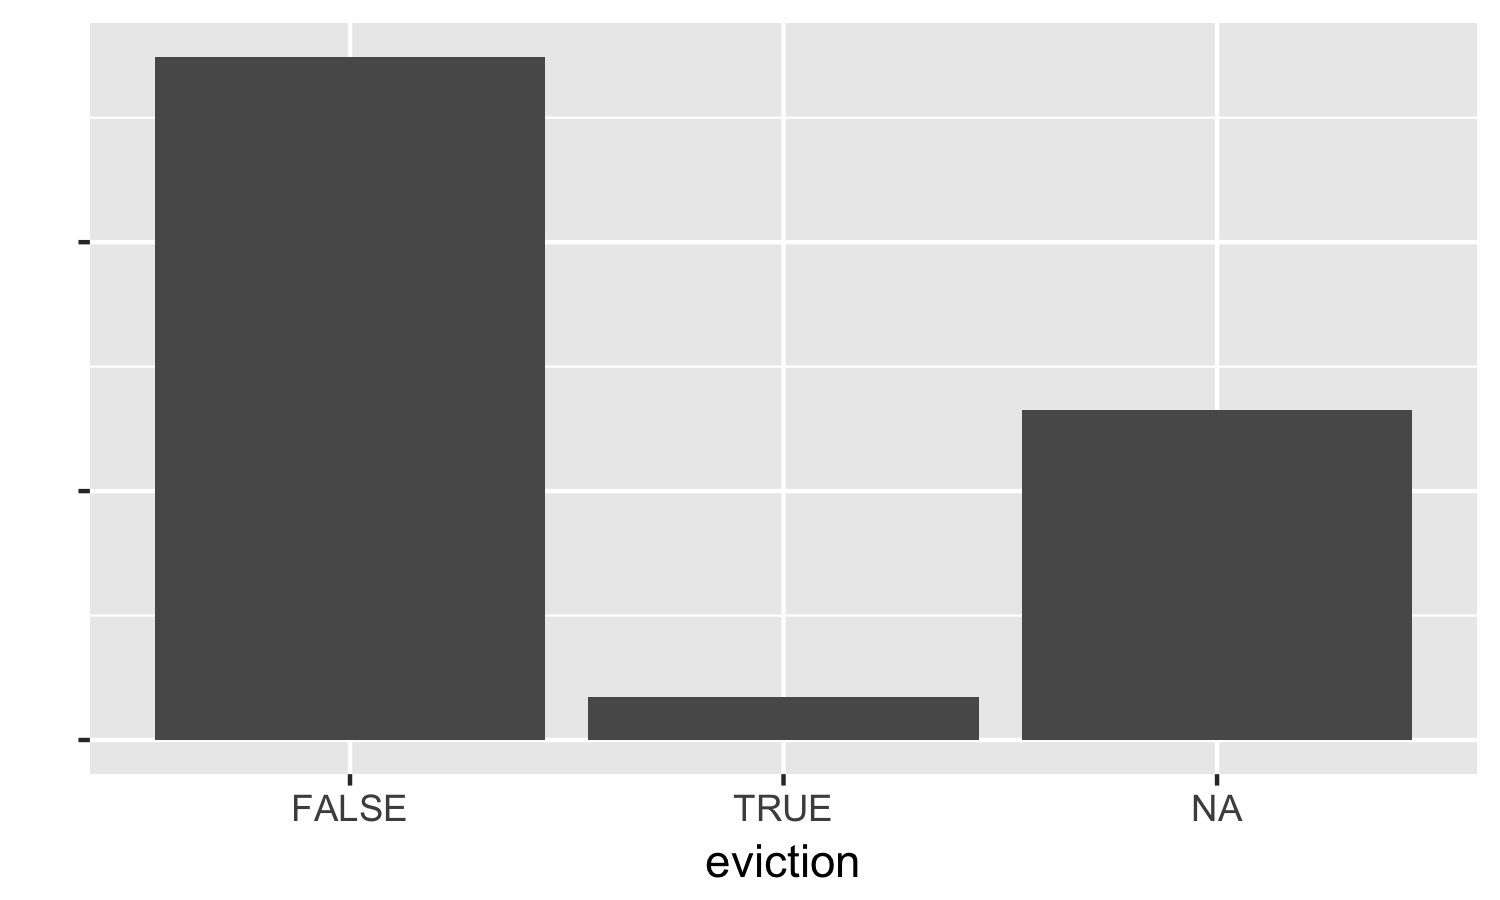
\includegraphics[width = .9\textwidth]{figures/evictionDist}

\end{frame}
%%%%%%%%%%%%%%%%%%%%%%%%%
\begin{frame}

\Large{
\begin{center}
Caregiver layoff\footnote{Learn more at \url{http://www.fragilefamilieschallenge.org/layoff/}\vskip .2cm}
\pause \vskip .5cm 
Does layoff of a caregiver \textbf{cause} collateral damage for kids?\footnote{Note: You will just create propensity scores for caregiver layoff given background variables; causal inference comes in the second stage of the Challenge when outcomes are measured several years from now.}
\end{center}
}

\end{frame}
%%%%%%%%%%%%%%%%%%%%%%%%%%%
\begin{frame}{Caregiver layoff}

\centering
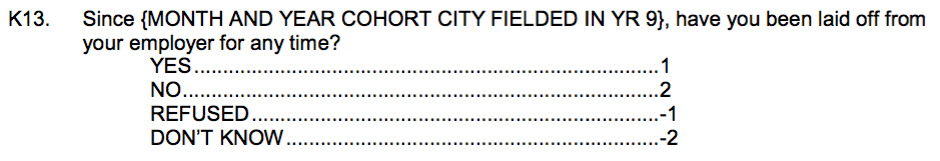
\includegraphics[width = .9\textwidth]{figures/layoff_questionnaire}

\end{frame}
%%%%%%%%%%%%%%%%%%%%%%%%%
\begin{frame}

\centering
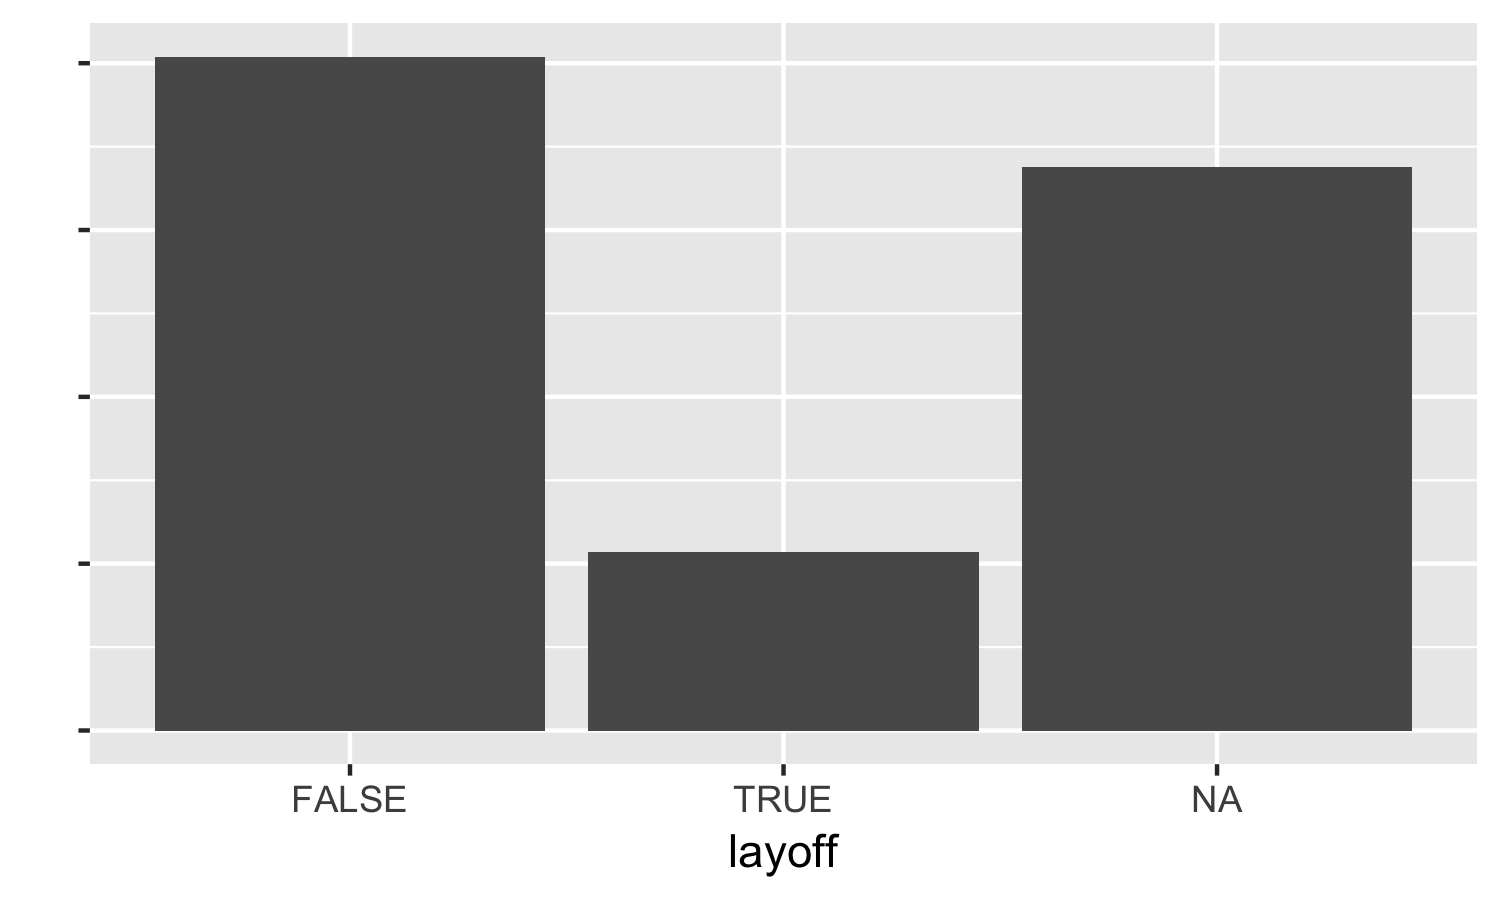
\includegraphics[width = .9\textwidth]{figures/layoffDist}

\end{frame}
%%%%%%%%%%%%%%%%%%%%%%%%%
\begin{frame}

\Large{
\begin{center}
Job training\footnote{Learn more at \url{http://www.fragilefamilieschallenge.org/job-training/}\vskip .2cm}
\pause \vskip .5cm 
Does job training for a caregiver \textbf{cause} collateral benefits for children?\footnote{Note: You will just create propensity scores for job training given background variables; causal inference comes in the second stage of the Challenge when outcomes are measured several years from now.}
\end{center}
}

\end{frame}
%%%%%%%%%%%%%%%%%%%%%%%%%%%
\begin{frame}{Caregiver job training}

\centering
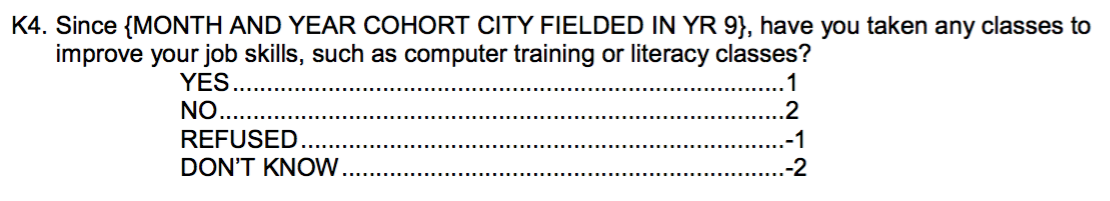
\includegraphics[width = .9\textwidth]{figures/jobTraining_questionnaire}

\end{frame}
%%%%%%%%%%%%%%%%%%%%%%%%%
\begin{frame}

\centering
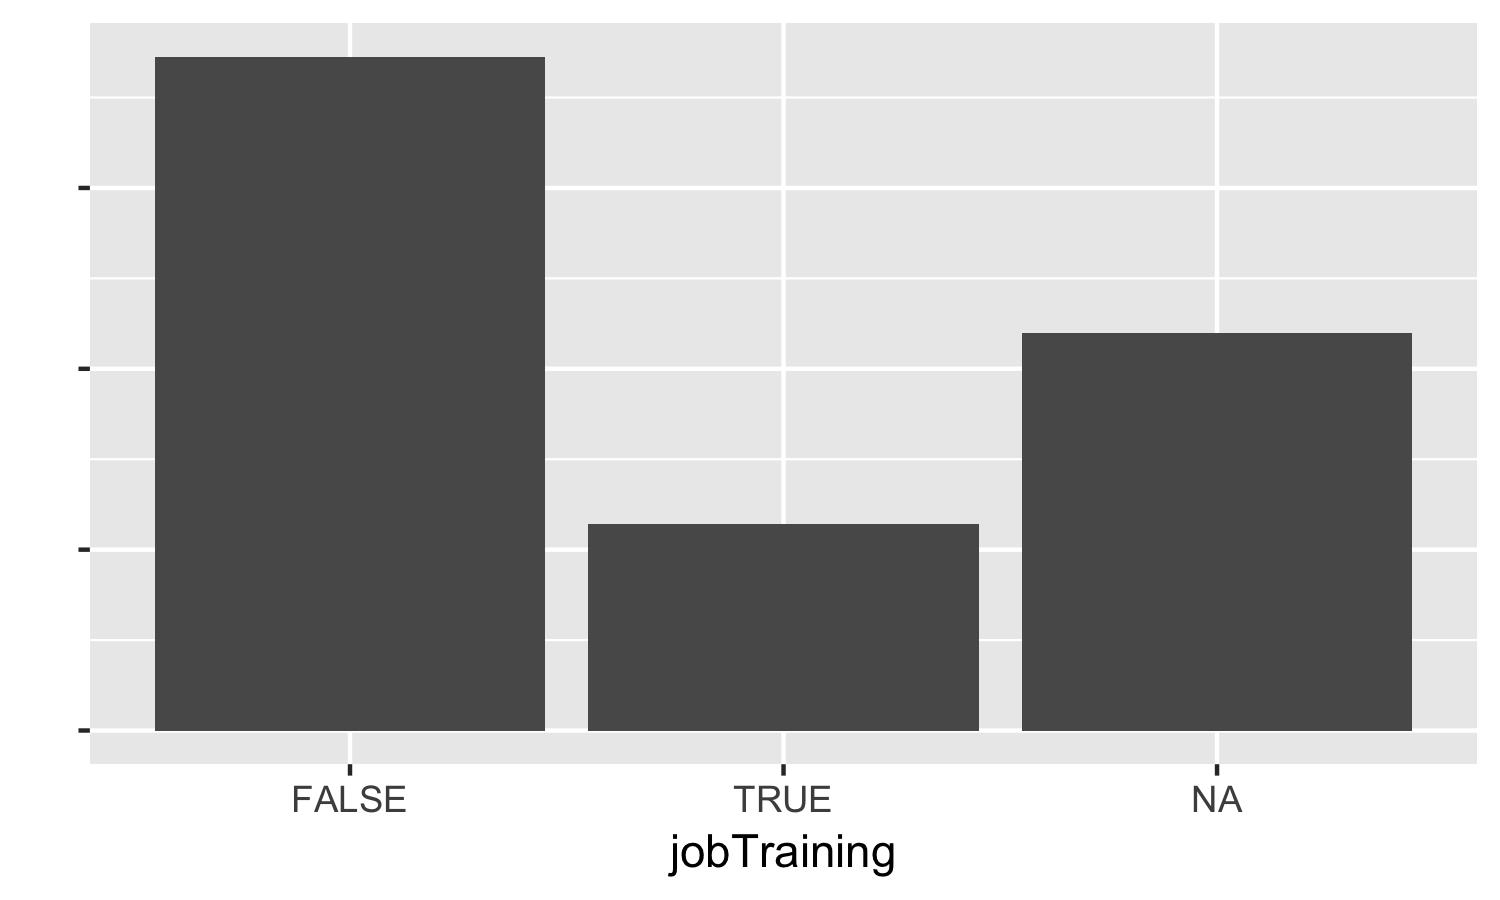
\includegraphics[width = .9\textwidth]{figures/jobTrainingDist}

\end{frame}
%%%%%%%%%%%%%%%%%%%%%%%%%%%
\begin{frame}

How do I know what the variables are? 
\begin{itemize}
\item Blog post: \textcolor{blue}{\href{www.fragilefamilieschallenge.org/survey-documentation/}{http://www.fragilefamilieschallenge.org/survey-documentation/}}
\item Fragile Families and Child Wellbeing Study website: \textcolor{blue}{\href{www.fragilefamilies.princeton.edu/}{http://www.fragilefamilies.princeton.edu/}}
\end{itemize}

\end{frame}
%%%%%%%%%%%%%%%%%%%%%%%%%%%
\begin{frame}

\centering
\includegraphics[width = .8\textwidth]{figures/Doc1}

\end{frame}
%%%%%%%%%%%%%%%%%%%%%%%%%%%
\begin{frame}

\centering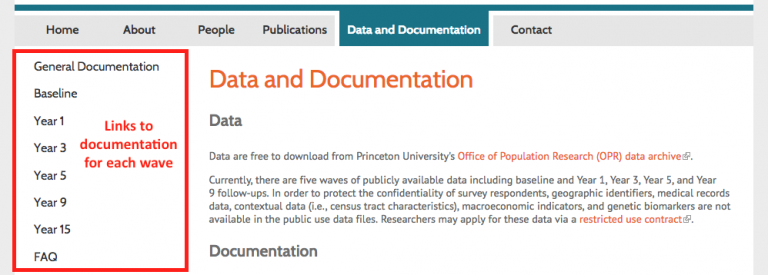
\includegraphics[width = .8\textwidth]{figures/Doc2}

\end{frame}
%%%%%%%%%%%%%%%%%%%%%%%%%%%
\begin{frame}

\centering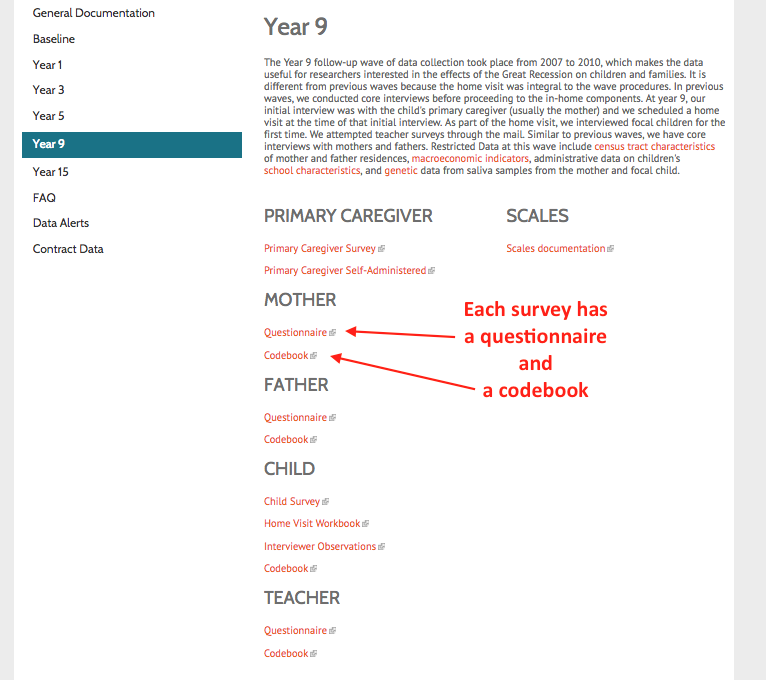
\includegraphics[width = .8\textwidth]{figures/Doc3}

\end{frame}
%%%%%%%%%%%%%%%%%%%%%%%%%%%
\begin{frame}

Questionnaire:\\
\centering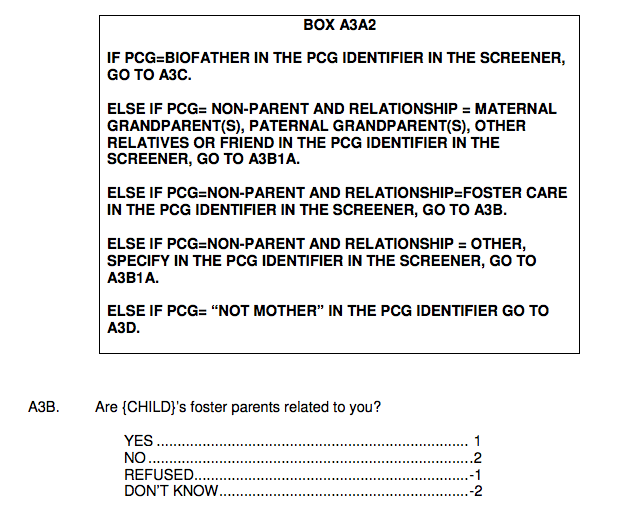
\includegraphics[width = .8\textwidth]{figures/Doc4}

\end{frame}
%%%%%%%%%%%%%%%%%%%%%%%%%%%
\begin{frame}

In the corresponding codebook, we see the count of respondents who gave each answer:
\vskip .3cm
\begin{center}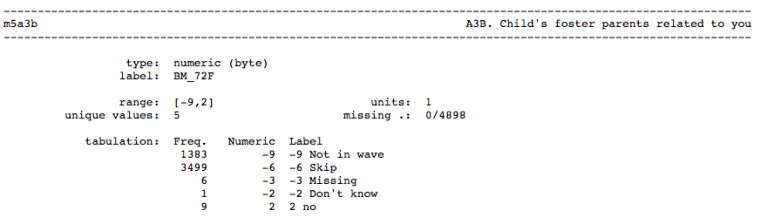
\includegraphics[width = .8\textwidth]{figures/Doc5}\end{center}
\vskip .3cm \pause
Things to note here:
\vskip .3cm \pause
\begin{itemize}
\item The question referred to in the questionnaire as A3B is called m5a3b in the codebook. \pause
\item There are missing codes.
\end{itemize}

\end{frame}
%%%%%%%%%%%%%%%%%%%%%%%%%%%
\begin{frame}

The general structure of the variable names is \vskip .5cm
\begin{scriptsize}[prefix for questionnaire type][wave number][question number]\end{scriptsize}

\end{frame}
%%%%%%%%%%%%%%%%%%%%%%%%%%%
\begin{frame}{Variable prefixes\footnote{For more info, see \url{http://www.fragilefamilieschallenge.org/survey-documentation/} \vskip .2cm}}

Common prefixes:

\begin{center}
\begin{scriptsize}
\begin{tabular}{cl}
Prefix & Meaning \\
\hline
m & Mother \\
f & Father \\
h or hv & Home visit \\
p & Primary caregiver \\
k & Kid (interview with the child) \\
kind\_ & Kindergarten teacher \\
t & Teacher \\
ffcc\_[something] & Child care surveys. \\
 & For a full list of the [something] see \href{http://fragilefamilies.princeton.edu/sites/fragilefamilies/files/ff_cc_notes.pdf}{\textcolor{blue}{this documentation}}.
\end{tabular}
\end{scriptsize}
\end{center}

\end{frame}
%%%%%%%%%%%%%%%%%%%%%%%%%%%
\begin{frame}{Constructed variables}

\begin{itemize}
\item Some variables are \alert{constructed} from several questions.
\item These tend to be important.
\item These variables add the additional prefix \alert{c} to the front of the variable name.
\item For instance, \texttt{cm1ethrace} indicates constructed mother's wave 1 race/ethnicity.
\end{itemize}

\end{frame}
%%%%%%%%%%%%%%%%%%%%%%%%%%%
\begin{frame}{Wave numbers $\neq$ child ages}

\begin{center}
\begin{tabular}{cc}
Wave number & Approximate child age \\
\hline
1 & 0, often called ``baseline'' \\
2 & 1 \\
3 & 3 \\
4 & 5 \\
5 & 9
\end{tabular}
\end{center}

\end{frame}
%%%%%%%%%%%%%%%%%%%%%%%%%%%
\begin{frame}{Common missing codes\footnote{For more complete list and explanation, see \url{http://www.fragilefamilieschallenge.org/missing-data/}\vskip .2cm}}

\begin{small}
\begin{itemize}
\item -9 Not in wave - Did not participate in survey/data collection component
\item -6 Valid skip - Intentionally not asked question; question does not apply to respondent or response known based on prior information.
\item -2 Don't know - Respondent asked question; responded ''Don't Know''.
\item -1 Refuse - Respondent asked question; refused to answer question
\item NA also used occasionally
\end{itemize}
\end{small}

\end{frame}
%%%%%%%%%%%%%%%%%%%%%%%%%%%
\begin{frame}{Getting the data}

\begin{enumerate}
\item Apply \begin{scriptsize}(\textcolor{blue}{\url{http://www.fragilefamilieschallenge.org/apply/}})\end{scriptsize}
\item Complete terms and conditions
\end{enumerate}

\end{frame}
%%%%%%%%%%%%%%%%%%%%%%%%%%%
\begin{frame}{Building a submission}

Submissions include:
\begin{enumerate}
\item Predictions
\item Code
\item Narrative explanation
\end{enumerate}

\vfill
Submission preparation instructions: \textcolor{blue}{\href{http://www.fragilefamilieschallenge.org/upload-your-contribution/}{www.fragilefamilieschallenge.org/upload-your-contribution/}}

\end{frame}
%%%%%%%%%%%%%%%%%%%%%%%%%%%
\begin{frame}{Get on the leaderboard}

\textcolor{blue}{\href{http://codalab.fragilefamilieschallenge.org/}{codalab.fragilefamilieschallenge.org}}\\
\vskip .2cm
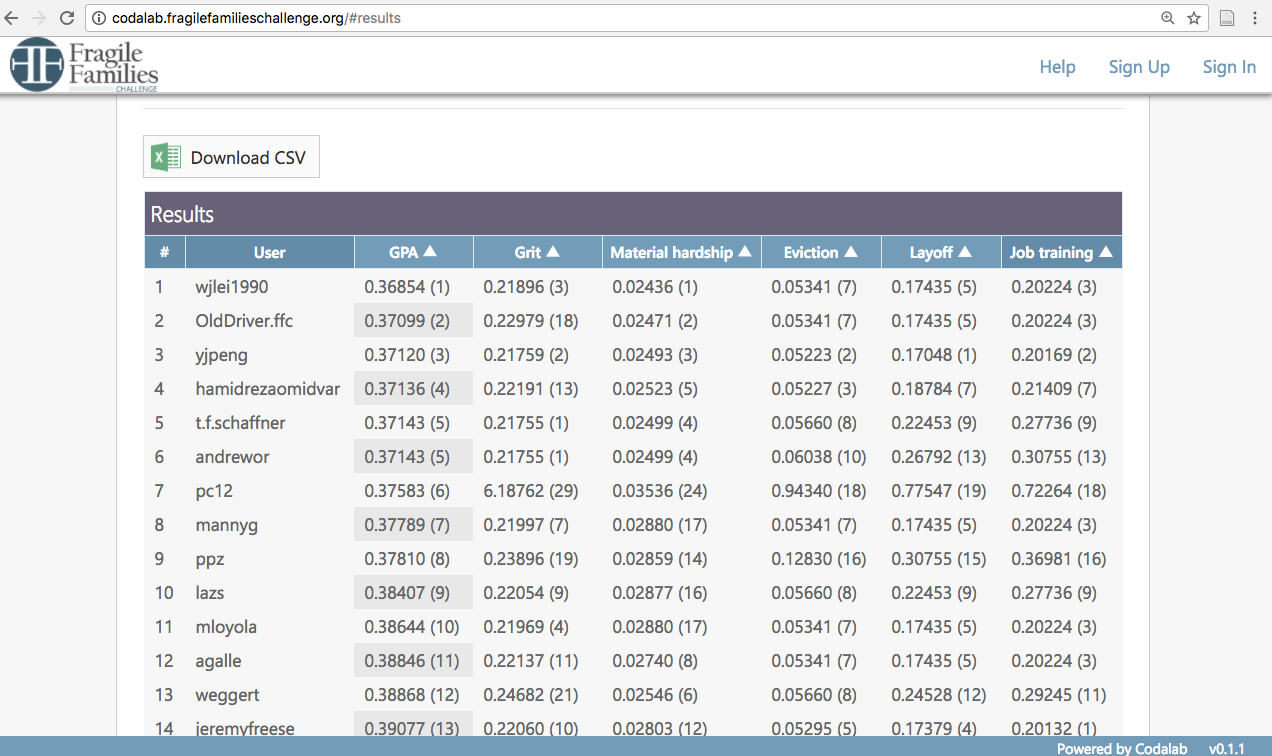
\includegraphics[width = .9\textwidth]{figures/leaderboard}

\end{frame}
%%%%%%%%%%%%%%%%%%%%%%%%%%%
\begin{frame}{Share ideas in the forum}

\textcolor{blue}{\href{http://codalab.fragilefamilieschallenge.org/}{codalab.fragilefamilieschallenge.org}}\\
\vskip .2cm
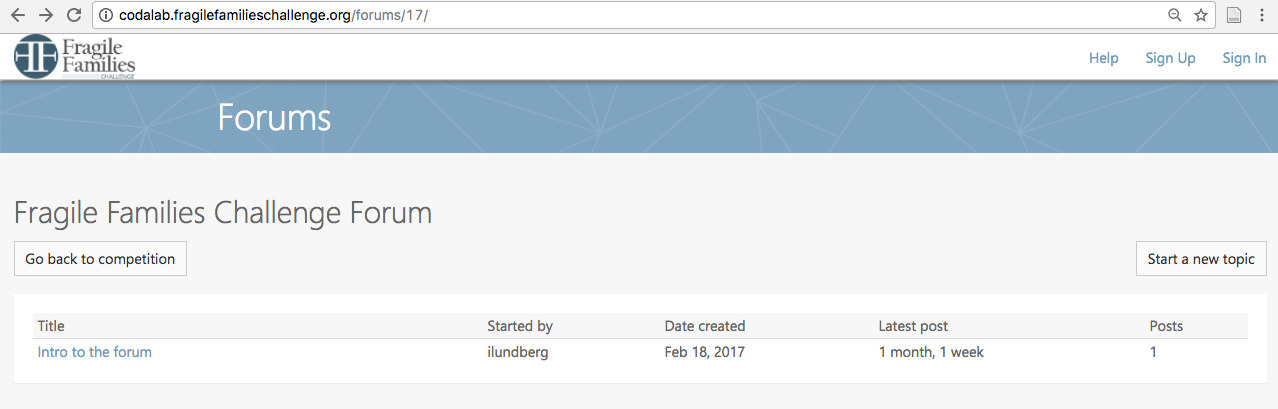
\includegraphics[width = .9\textwidth]{figures/forum}

\end{frame}
%%%%%%%%%%%%%%%%%%%%%%%%%%%
\begin{frame}{Share code open source on Github}

Participants have already contributed
\begin{itemize}
\item Code to support Stata users \begin{tiny}\textcolor{blue}{\url{https://github.com/fragilefamilieschallenge/stata-support}}\end{tiny}
\item Example submissions on which you can build \begin{tiny}\textcolor{blue}{\url{https://github.com/fragilefamilieschallenge/open-source-submissions}}\end{tiny}
\end{itemize}

\end{frame}
%%%%%%%%%%%%%%%%%%%%%%%%%%%
\begin{frame}

Why participate?
\begin{itemize}
\pause
\item care about the goals of the project
\pause
\item learn new skills
\pause
\item get involved in scientific research
\pause
\item win prizes
\pause
\item publish papers
\pause
\item have fun
\end{itemize}

\end{frame}
%%%%%%%%%%%%%%%%%%%%%%%%%%%
\begin{frame}

\begin{center}
\Large{\textcolor{blue}{\href{http://www.fragilefamilieschallenge.org}{www.fragilefamilieschallenge.org}}} 
\end{center}

\vfill

Questions? 
\begin{itemize}
\item Email: \href{mailto:fragilefamilieschallenge@gmail.com}{\textcolor{blue}{fragilefamilieschallenge@gmail.com}} 
\item Blog: \small{\textcolor{blue}{\href{http://www.fragilefamilieschallenge.org/blog-posts/}{www.fragilefamilieschallenge.org/blog-posts/}}}
\item Github: \small{\textcolor{blue}{\href{http://github.com/fragilefamilieschallenge}{www.github.com/fragilefamilieschallenge}}}
\item Forum: \small{\textcolor{blue}{\href{http://codalab.fragilefamilieschallenge.org}{codalab.fragilefamilieschallenge.org}}}
\end{itemize}

\end{frame}
%%%%%%%%%%%%%%%%%%%%%%%%%

\end{document}